\documentclass[twoside,a4paper,10pt]{report}
%%\usepackage[french]{babel} %% Use your own babel language
\usepackage[top=3cm,bottom=3cm,left=2.5cm,right=2.5cm]{geometry}
\usepackage{ucs}
\usepackage[utf8x]{inputenc}
\usepackage{pslatex}
\usepackage{hyperref}
\usepackage{graphicx}
\usepackage{tabularx}
\usepackage{supertabular}
\usepackage{pdflscape} %% Used for very big table
\usepackage{pdfpages} %% To add a cover to the doc
\usepackage{moreverb}
\usepackage{xcolor}
\usepackage{listings}
\usepackage{lastpage}
\usepackage{fancyhdr}
\usepackage{ulem}
\usepackage{textcomp}
\usepackage{wasysym}
\usepackage{sectsty}
\usepackage{wrapfig} %%Usefull for image 
%\usepackage{fguill} %%Use this package for guillemot[left|right] useless with babel set to french
\usepackage{eso-pic} %% Background
\pagestyle{fancy}%
\renewcommand{\headrulewidth}{0.1pt}
\renewcommand{\footrulewidth}{0pt}
\renewcommand{\chaptermark}[1]{%
	\markboth{\sffamily \chaptername\ \thechapter.\ #1}{}}

\renewcommand{\sectionmark}[1]{%
	\markright{{\sffamily #1}}{}}

\fancypagestyle{plain}{%
\fancyhf{}
\fancyfoot[R]{\thepage/\pageref{LastPage}}
\renewcommand{\headrulewidth}{0pt}
\renewcommand{\footrulewidth}{0pt}}
\fancyhf{}
\fancyhead[L]{\rightmark}
\fancyhead[R]{\leftmark}
\fancyfoot[R]{\thepage/\pageref{LastPage}}
\renewcommand{\headrulewidth}{0.1pt}
\renewcommand{\footrulewidth}{0pt}

\definecolor{Light}{gray}{.80}
\definecolor{Dark}{gray}{.20}

\newcommand{\key}[1]{\fcolorbox{Dark}{Light}{\textbf{#1}}}

\newcommand{\settexitref}[2]{(\ref{#1}p\pageref{#1})}
\newcommand{\dokutitlelevelone}[1]{\chapter{#1}}
\newcommand{\dokutitleleveltwo}[1]{\section{#1}}
\newcommand{\dokutitleleveltree}[1]{\subsection{#1}}
\newcommand{\dokutitlelevelfour}[1]{\subsubsection{#1}}
\newcommand{\dokutitlelevelfive}[1]{\paragraph{#1}}
\newcommand{\dokufootnote}[1]{\footnote{#1}}
\newcommand{\dokufootmark}[1]{\footnotemark[#1]}
\newcommand{\dokubold}[1]{\textbf{#1}}
\newcommand{\dokuitalic}[1]{\textsl{#1}}
\newcommand{\dokumonospace}[1]{\texttt{#1}}
\newcommand{\dokuunderline}[1]{\underline{#1}}
\newcommand{\dokuoverline}[1]{\sout{#1}}
\newcommand{\dokusupscript}[1]{\textsuperscript{#1}}
\newcommand{\dokusubscript}[1]{$_{#1}$}
\newcommand{\dokuhline}{\line(1,0){400}}
\newcommand{\dokulabel}[1]{\label{#1}}
\newcommand{\dokuitem}{\item}
\newcommand{\dokuquoting}{\textbar}
\newcommand{\dokutabularwidth}{\textwidth}
\newcommand{\dokusupertabularheadbreak}{\small\sl continued from previous page}
\newcommand{\dokusupertabulartailbreak}{\small\sl continued on next page}
\newcommand{\dokuheadingstyle}[1]{\textbf{#1}}
\definecolor{dokuheadingcolor}{rgb}{0,0,0.60}
\newcommand{\dokubackground}[1]{%
\AddToShipoutPicture{%
  \AtTextCenter{%
    \makebox(0,0)[c]{\resizebox{\textwidth}{!}{%
      \rotatebox{25}{\textsf{\textbf{\textcolor[gray]{0.90}{#1}}}}}}%
  }%
 }%
}

\graphicspath{{media/}}

\hypersetup{
pdftitle = {The Modular OpenRobots Simulation Engine - User guide},
pdfauthor = {LAAS-CNRS - ONERA},
pdfkeywords = {simulation, blender, robotics},
pdfcreator = {DokuTeXit},
pdfproducer = {dokuwiki + TeXit + pdflatex}
}
\title{The Modular OpenRobots Simulation Engine - User guide}
\author{LAAS-CNRS - ONERA}
\date{@DATE@}
\dokubackground{@BGTEXT@}
\begin{document}
\sffamily
\allsectionsfont{\sffamily}

\IfFileExists{cover.pdf}{
\includepdf[pages=-, fitpaper]{cover.pdf}
\thispagestyle{empty}
\cleardoublepage
}

\thispagestyle{empty}
\maketitle
\thispagestyle{empty}
\cleardoublepage
\tableofcontents
\newpage
\thispagestyle{plain}
\cleardoublepage
\newpage
%Rendering morse:user:summary





\dokutitlelevelone{Introducing the Modular OpenRobots Simulation Engine}
\label{55d4061a5aa52cfc82c5474279f29bd9}%% introducing_the_modular_openrobots_simulation_engine
\label{a80da1282f2c775bbc5f2c92c836968b}%%Start: summary => /home/slemaign/openrobots/data/pages/summary.txt

\begin{figure*}[h]
\centering

\includegraphics[width=50pt]{openrobots-simulator.png}
\caption{Logo MORSE}
\end{figure*}


Welcome to the official documentation for the MORSE project.

For an global description of the project, consult the 
\href{http://homepages.laas.fr/gechever/Documents/morse-21062010.pdf}{ article}
submitted to the \href{http://www.simpar.org/}{ Simpar 2010} conference.

This first section will help you to find your way into the MORSE documentation.


\dokutitleleveltwo{What is MORSE?}
\label{cb90401e2d53fdeab390406232e6c72f}%% what_is_morse

\begin{figure*}[h]
\raggedleft
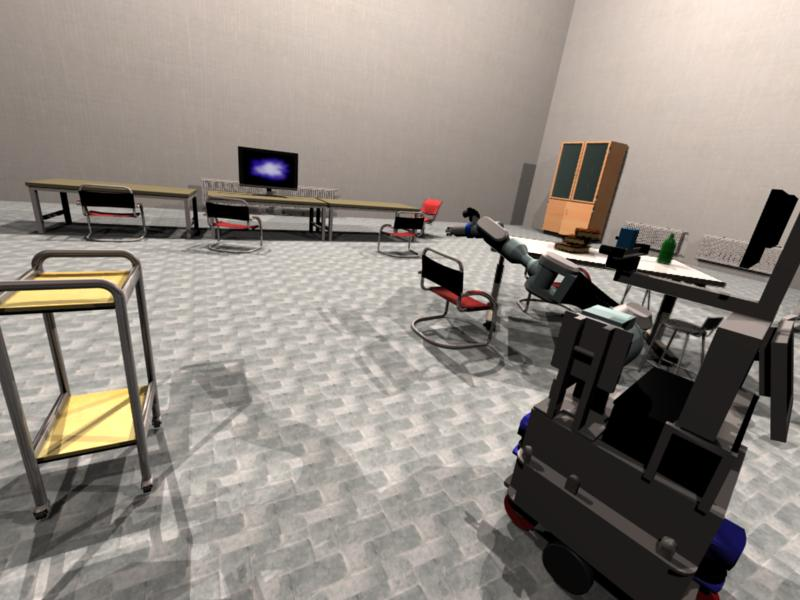
\includegraphics[width=300pt]{simu_render_indoors.jpg}
\caption{Introducing MORSE}
\end{figure*}




\begin{itemize}
\dokuitem  A versatile simulator for \dokubold{generic mobile robots simulation} (single or multi robots),
\dokuitem  Enabling \dokubold{realistic} and \dokubold{dynamic} environments (with other interacting agents -humans- or objects), 
\dokuitem  Don't reinvent the wheel: critical components reused from other open source projects (\dokubold{Blender} for 3D rendering + physical simulation + UI, dedicated robotic middlewares for communications + robot hardware support),
\dokuitem  \dokubold{Seamless workflow}: since the simulator rely on Blender for both modeling and the real time 3D engine, creating and modifying a simulated scene is straightforward.
\dokuitem  Entirely scriptable in \dokubold{Python},
\dokuitem  Adaptable to various \dokubold{level of simulation realism} (for instance, we may want to simulate exteroceptive sensors like cameras in certain cases and access directly to a higher level representation of the world -like labeled artifacts- in other cases),
\dokuitem  Currently compatible with \dokubold{YARP} and LAAS OpenRobots robotics frameworks,
\dokuitem  Fully open source, BSD-compatible.
\end{itemize}

\begin{figure*}[h]
\centering
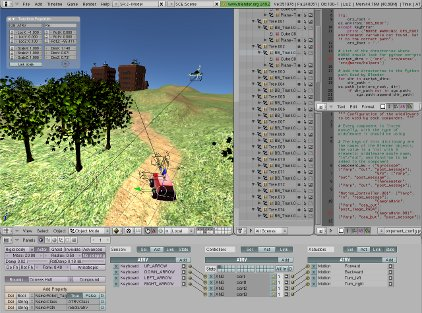
\includegraphics[width=300pt]{outdoor_example.jpg}
\caption{An ATRV in an outdoor scenario}
\end{figure*}



\dokutitleleveltwo{Getting started}
\label{46b862bd16703034ef594b2996ec8166}%% getting_started

\begin{enumerate}\dokuitem  \hyperref[ea09bb364ef1bffd889e76b7a59035fc]{ Install MORSE}
\dokuitem  \hyperref[60efe788544a384827c39a9803dab85b]{ Check the MORSE command reference}
\dokuitem  \hyperref[0575c8d592fb7b088226750aceec2b4e]{ Jump to the tutorial}
\end{enumerate}

\dokutitleleveltwo{The MORSE Workflow}
\label{2963f1f90771a121484ee5fd4a4251c0}%% the_morse_workflow

Discover the MORSE workflow: how to build a complete simulation scenario, from 
the creation of a custom robot with predefined sensors and actuators to the 
complete scene, including other robots or humans.

\hyperref[514bac84019bd5e09c0e2b525b09f429]{ Go to: the typical MORSE workflow}


\dokutitleleveltwo{Components library \& Supported middlewares}
\label{0c88d1b20b693084703691e13ff5151f}%% components_library_supported_middlewares

\begin{itemize}
\dokuitem  MORSE offers a set of predefined sensors and controllers that cover basic simulation needs in robotics. To know how to add new components, please refer to the developer documentation.
\end{itemize}

The following page lists all the currently existing components and their properties:

\hyperref[004fdec0cc1a00c19c57e892b7eb1400]{ Go to: the MORSE component library}



\begin{itemize}
\dokuitem  The output (or input) of the simulator can be altered (for instance to add noise) by so called modifiers.
\end{itemize}

\hyperref[25bc6523e9298f4691b3c8200a395d92]{ Go to: Data modifiers}



\begin{itemize}
\dokuitem  MORSE relies on \dokuitalic{middlewares} to integrate in your robotic architecture.
\end{itemize}

We currently support only \dokubold{\href{http://eris.liralab.it/yarp/}{ YARP}}, 
\dokubold{\href{https://softs.laas.fr/openrobots/wiki/pocolibs}{pocolibs}} and a simple 
text-based socket protocol. More middlewares are expected to be added in the 
next versions.

\hyperref[9a05db9c4b60b0527010fd997682f523]{ Go to: Middleware support}


\dokutitleleveltwo{Advanced tutorials}
\label{1db3103f04a8f50e1168ef3c23748f71}%% advanced_tutorials

\hyperref[1db3103f04a8f50e1168ef3c23748f71]{ List of all tutorials}


\dokutitleleveltree{Setting up a YARP-based simulation}
\label{a3bba0b321b28de69351875f85d854db}%% setting_up_a_yarp-based_simulation

This tutorial shows a simple scenario with Yarp: Simple dummy autonomous navigation towards a user-given target (x,y). 
The robots becomes red when it intersects obstacles or bounces on them. Use the same example as the quick start ? 
(sole difference: the goal is given through YARP, sensor data are exported with YARP  maybe add a camera, since it is trivial to display an image with YARP).

\hyperref[1dd029a60f7f3dd1deaf993ce4538edf]{ Go to: YARP-based simulation tutorial}

%Rendering morse:user:installation
\dokutitlelevelone{MORSE installation}
\label{1d96fd68defedd8a755f2a95c80e618f}%% morse_installation
\label{ea09bb364ef1bffd889e76b7a59035fc}%%Start: installation => /home/slemaign/openrobots/data/pages/installation.txt

\dokutitleleveltwo{Requirements - What you need to install before}
\label{27060cbab4a02c4805c03a15b2aad7d7}%% requirements_-_what_you_need_to_install_before

\dokutitleleveltree{Hardware}
\label{3ca14c518d1bf901acc339e7c9cd6d7f}%% hardware

To display textures correctly in the simulator, as well as to generate images using the simulated cameras, you will need to have a graphics card that supports GLSL shading. The Blender website lists these graphic cars as compatible with GLSL:


\begin{itemize}
\dokuitem  ATI Radeon 9{\texttimes}00, Xx00, X1x00, HD2x00 and HD3x00 series and newer.
\dokuitem  NVidia Geforce FX, 6{\texttimes}00, 7{\texttimes}00, 8{\texttimes}00, 9{\texttimes}00 and GTX 2{\texttimes}0 and newer.
\end{itemize}

\dokutitleleveltree{Required software}
\label{accfa4c836a5caff827d9adbf6bea7dc}%% required_software

\begin{itemize}
\dokuitem  Python (2.6 or +)
\dokuitem  Blender 2.49 build with Python 2.6 \dokufootnote{For the moment the simulator works only with this version. Blender 2.5 is being worked on.}
\dokuitem  git to get the code of the simulator:
\end{itemize}

\small
\begin{verbatimtab}
$ git clone http://trac.laas.fr/git/robots/morse.git
\end{verbatimtab}
\normalsize

If you plan to use the simulator with raw sockets of text files as "middleware",
you don't need anything else. Otherwise, you need to install the software for other middlewares.


\dokutitleleveltree{YARP}
\label{ec46d0b85077d7a7fe8da2e2b4c70462}%% yarp

For the YARP bindings


\begin{itemize}
\dokuitem  YARP version (2.2.5 or +)
\dokuitem  YARP python binding
\dokuitem  ACE ( 5.6.3 or +, required for YARP)
\end{itemize}

Instructions to create YARP-Python bindings are \href{http://eris.liralab.it/wiki/YARP_and_Python}{ here}.

Note that the easiest way to install YARP is probably to use \dokumonospace{robotpkg} (see \href{http://homepages.laas.fr/mallet/robotpkg}{ robotpkg homepage} for more informations). Follow the instructions on installing \dokumonospace{robotpkg}. Then add the environment variable \dokumonospace{ROBOTPKG{\textunderscore}BASE} to your shell.
Then to install \dokumonospace{YARP}:


\small
\begin{verbatimtab}
$ cd $ROBOTPKG_BASE/robotpkg/architecture/yarp
$ make update
\end{verbatimtab}
\normalsize
Afterwards, install the YARP python bindings bindings:


\small
\begin{verbatimtab}
$ cd $ROBOTPKG_BASE/robotpkg/devel/libpyyarp
$ make update
\end{verbatimtab}
\normalsize

Compiling the YARP Python binding will create two files: \dokumonospace{yarp.py} and \dokumonospace{{\textunderscore}yarp.so}, and install them in\\ \dokumonospace{{\textdollar}ROBOTPKG{\textunderscore}BASE/lib/python2.6/site-packages/}
You'll need to set the environment variable \dokumonospace{PYTHONPATH} to \dokumonospace{{\textdollar}ROBOTPKG{\textunderscore}BASE/lib/python2.6/site-packages/} to let python find the YARP module.

If you are not using robotpkg to install YARP, then make sure to copy the files \dokumonospace{yarp.py} and \dokumonospace{{\textunderscore}yarp.so} to your Python lib directory (\dokumonospace{/usr/lib/python2.6/site-packages/}) or at some place reachable from your \dokumonospace{PYTHONPATH} environment variable.


\dokutitleleveltree{Pocolibs}
\label{15f13a3fccdd1ef095539316b61c03c8}%% pocolibs

To build Pocolibs bindings (the LAAS-CNRS middleware), you need to install Pocolibs on your system.

The recommended way to do it is through \dokumonospace{robotpkg} (see \href{http://homepages.laas.fr/mallet/robotpkg}{ robotpkg homepage} for more informations).

To install:


\small
\begin{verbatimtab}
$ cd $ROBOTPKG_BASE/robotpkg/devel/pocolibs
$ make update
\end{verbatimtab}
\normalsize

\dokutitleleveltwo{Installation}
\label{ea09bb364ef1bffd889e76b7a59035fc}%% installation

From your MORSE root directory:


\small
\begin{verbatimtab}
$ mkdir build && cd build
$ cmake ..
\end{verbatimtab}
\normalsize

By default, MORSE will install in \dokumonospace{/usr/local}. You can easily change that by launching ccmake instead of cmake.
When using ccmake, it is also possible to select the optional middleware bindings for YARP and Pocolibs.
You can set up the different variables using the command line:


\begin{itemize}
\dokuitem  \dokumonospace{CMAKE{\textunderscore}INSTALL{\textunderscore}PREFIX} controls where will be installed MORSE. Note: The install prefix directory will be referred to as \dokumonospace{{\textdollar}ORS{\textunderscore}ROOT} in this document.
\dokuitem  \dokumonospace{BUILD{\textunderscore}POCOLIBS{\textunderscore}SUPPORT} controls the build of pocolibs support in MORSE
\dokuitem  \dokumonospace{BUILD{\textunderscore}YARP2{\textunderscore}SUPPORT} controls the build of YARP support in MORSE
\dokuitem  \dokumonospace{CMAKE{\textunderscore}BUILD{\textunderscore}TYPE} controls the optimization stuff for C/C++ extension (Release is a good choice).
\end{itemize}

\small
\begin{verbatimtab}
$ make install
\end{verbatimtab}
\normalsize

To build and install MORSE with YARP support in \dokumonospace{/opt}, you need something like:


\small
\begin{verbatimtab}
$ cmake -DBUILD_YARP2_SUPPORT=ON -DCMAKE_BUILD_TYPE=Release -DCMAKE_INSTALL_PREFIX=/opt ..
\end{verbatimtab}
\normalsize

Two environment variables must be set to let the simulator know where to look for the installed components:



\begin{itemize}
\dokuitem  \dokumonospace{{\textdollar}PYTHONPATH} specifies the directories where MORSE scripts are located.  It will start with the MORSE installation prefix, followed by the path to the python scripts. It must also include the full path to the directory \dokumonospace{morse/blender} within the installed files. Example:
\end{itemize}

\small
\begin{verbatimtab}
tcsh:
setenv PYTHONPATH
$ORS_ROOT/lib/python2.6/site-packages:$ORS_ROOT/lib/python2.6/site-packages/morse/blender
\end{verbatimtab}
\normalsize

\small
\begin{verbatimtab}
bash:
export
PYTHONPATH=$ORS_ROOT/lib/python2.6/site-packages:$ORS_ROOT/lib/python2.6/site-packages/morse/blender
\end{verbatimtab}
\normalsize

\begin{itemize}
\dokuitem  {\textdollar}ORS{\textunderscore}BLENDER that allows you to specify a custom Blender executable (else, Blender is looked for in the path).
\end{itemize}

\dokutitleleveltwo{Running a simulation}
\label{70cc733d625ccafb4d56ea8f7dcb7973}%% running_a_simulation

[YARP specific] Before starting a simulation: Start the YARP's server using this command in a separate terminal:


\small
\begin{verbatimtab}
$ yarp server
\end{verbatimtab}
\normalsize

Launch MORSE by calling the morse executable:


\small
\begin{verbatimtab}
$ morse
\end{verbatimtab}
\normalsize

Several options are available, check them with:


\small
\begin{verbatimtab}
$ morse help
\end{verbatimtab}
\normalsize

You can check your configuration is ok with:


\small
\begin{verbatimtab}
$ morse check
\end{verbatimtab}
\normalsize

Once launched, you can test the simulator by loading one of the example scenarii from\\ \dokumonospace{{\textdollar}ORS{\textunderscore}ROOT/share/morse/examples/scenarii} (.blend files)

To start a simulation, go on Blender and press \key{P} to play the scenario.


\dokutitleleveltwo{Testing}
\label{ae2b1fca515949e5d54fb22b8ed95575}%% testing

To test the external control clients:


\begin{itemize}
\dokuitem  Open the Blender file: \dokumonospace{{\textdollar}ORS{\textunderscore}ROOT/share/morse/examples/scenarii/example-1-solved.blend}
\dokuitem  Start the simulation \key{P}
\dokuitem  On a separate terminal, run the Python program:
\end{itemize}
  {\textdollar} python {\textdollar}ORS{\textunderscore}ROOT/share/morse/examples/clients/atrv/socket{\textunderscore}v{\textunderscore}omega{\textunderscore}client.py


\begin{itemize}
\dokuitem  Follow the client program's instructions to send movement commands to the robot and to read information back
\dokuitem  To finish the simulation, press \key{Esc}
\dokuitem  To close Blender, press \key{Ctrl + Q}, and then \key{Enter}
\end{itemize}

Tips: If you have any problem to start to play a simulation: start blender
from a terminal and send the error messages to morse{\textunderscore}dev@laas.fr.

%Rendering morse:user:basic_morse
\dokutitlelevelone{Getting started: basic MORSE usage}
\label{cef0f135a902b28b4a51575ed8a2cec1}%% basic_morse_usage
\label{60efe788544a384827c39a9803dab85b}%%Start: basic_morse => /home/slemaign/openrobots/data/pages/basic_morse.txt

\dokutitleleveltwo{Basic Blender commands}
\label{7809ce8524191dac30521dd680b9a379}%% basic_blender_commands

The setup and configuration of a simulation scenario in MORSE is completely done using the Blender interface. It is very particular and different from almost any other computer program.
A good explanation on the use of Blender's interface can be found \href{http://en.wikibooks.org/wiki/Blender_3D:_Noob_to_Pro/Learning_Graphic_Interface}{ here}.
Here we present the most useful commands necessary to operate MORSE


\dokutitleleveltree{Selection of an object}
\label{d461f4bc8beb6b0a8442d6d4da3a0c6d}%% selection_of_an_object

\includegraphics[height=1em]{RMB.png} over the object

Pressing \key{A} will toggle selection of all or none of the objects in the current scene.


\dokutitleleveltree{Geometric transformations of an object}
\label{001ad77ecf37a2b719f6d1a347faed00}%% geometric_transformations_of_an_object

\dokutitlelevelfour{Keyboard input}

To enter with the keyboard accurate transformation value, press \key{N} to display the \dokubold{Transfor Properties} sub-window of the selected object. Then change the values of the \dokubold{Loc}, \dokubold{Rot} or \dokubold{Scale} fields.


\dokutitlelevelfour{With the mouse}
The shortcut keys are \key{G} for translation, \key{S} for scaling and
 \key{R} for rotation.

Press the desired key, then move with the mouse.

Press 
\includegraphics[height=1em]{LMB.png} to accept transformation, or 
\includegraphics[height=1em]{RMB.png} to cancel.

Tips:


\begin{itemize}
\dokuitem  Hold \key{Ctrl} key while transforming, to use discrete intervals. 
\dokuitem  Press \key{X}, \key{Y} or \key{Z} to constraint the transformation on one axis.
\end{itemize}

\dokutitleleveltree{Camera view shortcuts}
\label{490b5cdd607bc3b8891df904de25d417}%% camera_view_shortcuts
Use the numeric keyboard


\begin{itemize}
\dokuitem  Top view: \key{'7 NumPad'}
\dokuitem  Front view: \key{'1 NumPad'}
\dokuitem  Side view: \key{'3 NumPad'}
\dokuitem  Main camera view: \key{'0 NumPad'}
\dokuitem  Toggle perspective/orthogonal view: \key{'5 NumPad'}
\end{itemize}

The view of the scene can also be adjusted manually by holding down 
\includegraphics[height=1em]{MMB.png} and moving the mouse


\dokutitleleveltree{Switch shading modes}
\label{930ca388b865b6b10e3f5eb29f9bb084}%% switch_shading_modes

\begin{itemize}
\dokuitem  Wireframe/solid: \key{Z}
\dokuitem  Wireframe/solid: \key{Shift + Z}
\dokuitem  Solid/textured: \key{Alt + Z}
\end{itemize}

\dokutitleleveltree{Opening and saving files}
\label{0b2dd5c17c378b3048db1b45587a2d17}%% opening_and_saving_files

\begin{itemize}
\dokuitem  Open file: \key{F1}
\dokuitem  Save file: \key{Ctrl + W}
\dokuitem  Save file as\ldots{} : \key{F2}
\dokuitem  Quit Blender: \key{Ctrl + Q}
\end{itemize}

\dokutitleleveltree{Button panels}
\label{626500a59dae6683d1d105511ef0622a}%% button_panels
Selection of the type of panel in the Buttons Window:


\begin{itemize}
\dokuitem  Logic buttons: \key{F4}
\dokuitem  Material buttons: \key{F5}
\dokuitem  Texture buttons: \key{F6}
\dokuitem  Object buttons: \key{F7}
\dokuitem  Editing buttons: \key{F9}
\end{itemize}

\dokutitleleveltwo{MORSE camera view and control}
\label{1a5ca2519d76146bd4b2f974b54811d3}%% morse_camera_view_and_control
A simulation in MORSE is executed using the Game Engine mode of Blender. When in this mode, the button panels of Blender are disabled and the controls change.
It is recommended to switch the Blender 3D View window to full screen before starting a simulation. Press \key{Ctrl + {$\uparrow$}} when the mouse is over a window to toggle it to full screen and back.

During simulation, the view of the scene is controlled using the mouse and keyboard, in the same way as First Person Shooter game.The camera can be moved around using:


\begin{itemize}
\dokuitem  \key{W}, \key{S} to move forward and backward
\dokuitem  \key{A}, \key{D} to move left and right
\dokuitem  \key{Q}, \key{E} to move up and down
\end{itemize}
The direction the camera points to is controlled with the mouse.

It is possible to adjust the speed of the movement, by selecting the \dokumonospace{CameraFP} object in the scene, and adjusting the properties \dokubold{Sensitivity} for the mouse, and \dokubold{Speed} for the keyboard.


\dokutitleleveltwo{Creation of scenario files}
\label{477e85464263e092bdd386389bab76b2}%% creation_of_scenario_files

Use the \dokumonospace{morse} binary program, to open or create new simulation scenarios:



\small
\begin{verbatimtab}
$ morse
\end{verbatimtab}
\normalsize

Will create a new copy of the basic scenario file, ready to be modified.



\small
\begin{verbatimtab}
$ morse create [Filename]
\end{verbatimtab}
\normalsize

It will create a new file with the name given, and ready to be edited.



\small
\begin{verbatimtab}
$ morse [Filename]
\end{verbatimtab}
\normalsize

The MORSE simulator is started using an existing file with the name specified.


\dokutitleleveltwo{Adding components to files}
\label{94afd3e6d92cbe0e7c018d7a85463367}%% adding_components_to_files

\begin{itemize}
\dokuitem  Open file
\dokuitem  Link elements (robots, scenarios sensors) \key{Shift + F1}
\dokuitem  Select the source Blender file, and then Objects
\dokuitem  Select the objects to insert, using the 
\includegraphics[height=1em]{RMB.png}
\dokuitem  Select the \dokubold{Link} and \dokubold{Relative Paths} toggle buttons
\dokuitem  Click \dokubold{Load Library}
\dokuitem  The objects will be inserted in the scene, at the origin, and with a cyan selection highlight
\dokuitem  Select the parent object, then press \key{Shift + G}, then select \dokubold{Children} or press \key{Enter}
\dokuitem  Press the \key{L} key, then select \dokubold{Selected Objects} or press \key{Enter}
\dokuitem  The object will now have a pink selection highlight, and can be moved/rotated/scaled
\end{itemize}

\dokutitleleveltwo{Parenting components to a robot}
\label{5c8528e5d80c7c0537856e0911e6cdc8}%% parenting_components_to_a_robot

\begin{itemize}
\dokuitem  Select the Empty object of the component, then hold \key{Shift} and select the robot
\dokuitem  Press \key{Ctrl + P}, then select \dokubold{Make parent} or press \key{Enter}
\end{itemize}

\dokutitleleveltwo{Start and stop a simulation}
\label{466b971dc2d338787d665353c2a0f40a}%% start_and_stop_a_simulation

To start the simulation, press the \key{P} key.

To stop, press the \key{Esc} key.


\includegraphics[height=1em]{attention.png} Under certain error conditions ESC may not work, in that case, an emergency exit
key is \key{F12}, which will try to exit without doing executing the 
cleanup functions. If this doesn't work, the command \key{Ctrl + \\} on the 
terminal will kill Blender.

%Rendering morse:user:tutorial
\dokutitlelevelone{Tutorial example}
\label{d0e1bed8b40ec8e4f9cc0cc0a11ff110}%% tutorial_example
\label{0575c8d592fb7b088226750aceec2b4e}%%Start: tutorial => /home/slemaign/openrobots/data/pages/tutorial.txt

This tutorial assumes MORSE is properly installed. If not, follow the instructions \hyperref[ea09bb364ef1bffd889e76b7a59035fc]{ here}.


\dokutitleleveltwo{Setup of the simulation scene}
\label{80527725485ea9e7bedbc9d918895a02}%% setup_of_the_simulation_scene

\dokutitleleveltree{Load sample file}
\label{4238ab1e3d8f80f2fdec7f34e17e0f67}%% load_sample_file

Open the MORSE simulator with the test file provided with the installation, by using this command:



\small
\begin{verbatimtab}
$ morse $ORS_ROOT/share/morse/examples/scenarii/example-1.blend
\end{verbatimtab}
\normalsize

This will load a scene with a robot in a room with some furniture.


\dokutitleleveltree{Link an actuator}
\label{81c6b973417d3e5000d27d9c1c805b96}%% link_an_actuator

We'll add a motion controller to the robot, so that it can receive commands from an external program. The robot will then move according to the instructions received. In this case we'll add a controller that uses linear and angular speed (V, W).



\begin{enumerate}\dokuitem  With the mouse over the 3D view in Blender, press \key{Shift + F1} to open the Load Library browser
\dokuitem  Navigate to the directory \dokumonospace{{\textdollar}ORS{\textunderscore}ROOT/data/morse/components/controllers}
\dokuitem  Press 
\includegraphics[height=1em]{LMB.png} over the file \dokumonospace{morse{\textunderscore}vw{\textunderscore}control.blend}
\dokuitem  Press 
\includegraphics[height=1em]{LMB.png} over the item \dokumonospace{Object}
\dokuitem  Toggle the buttons \dokubold{Relative Paths} and \dokubold{Link} at the bottom of the window
\dokuitem  Press 
\includegraphics[height=1em]{RMB.png} over the item \dokumonospace{Motion{\textunderscore}Controller}
\dokuitem  Press the button \dokubold{Load Library}. You'll return to the 3D View
\dokuitem  Select the newly inserted object in the scene, either by 
\includegraphics[height=1em]{RMB.png} clicking over the object in the 3D View, or 
\includegraphics[height=1em]{LMB.png} over the object's name in the Outliner window. The object will be highlighted in cyan color, and can not be moved around.
\dokuitem  Convert the object to local, by pressing \key{L} then hitting \key{Enter}
\dokuitem  With the controller selected, hold down \key{Shift} and then 
\includegraphics[height=1em]{RMB.png} over the robot object
\dokuitem  Press \key{Ctrl + P} and then hit \key{Enter} make the robot the parent of the controller
\end{enumerate}

\dokutitleleveltree{Link a Gyroscope sensor}
\label{f019fe80659ff060e77872347a3add5c}%% link_a_gyroscope_sensor

Next we'll add a sensor to the robot that will report the angles of the robot orientation with respect to the reference axes (yaw, pitch and roll)



\begin{enumerate}\dokuitem  With the mouse over the 3D view in Blender, press \key{Shift + F1} to open the Load Library browser
\dokuitem  Navigate to the directory \dokumonospace{{\textdollar}ORS{\textunderscore}ROOT/data/morse/components/sensors}
\dokuitem  Press 
\includegraphics[height=1em]{LMB.png} over the file \dokumonospace{morse{\textunderscore}gyroscope.blend}
\dokuitem  Press 
\includegraphics[height=1em]{LMB.png} over the item \dokumonospace{Object}
\dokuitem  Toggle the buttons \dokubold{Relative Paths} and \dokubold{Link} at the bottom of the window
\dokuitem  Press 
\includegraphics[height=1em]{RMB.png} over the items \dokumonospace{Gyroscope} and \dokumonospace{Gyro{\textunderscore}box}
\dokuitem  Press the button \dokubold{Load Library}. You'll return to the 3D View
\dokuitem  Select the newly inserted \dokumonospace{Gyroscope} object in the scene, either by 
\includegraphics[height=1em]{RMB.png} clicking over the object in the 3D View, or 
\includegraphics[height=1em]{LMB.png} over the object's name in the Outliner window. The object will be highlighted in cyan color, and can not be moved around.
\dokuitem  Select the child object, by pressing \key{Shift + G}, then hitting \key{Enter}
\dokuitem  Convert the object to local, by pressing \key{L} then hitting \key{Enter}
\dokuitem  Switch to front view by pressing \key{'1 NumPad'}
\dokuitem  Press \key{G}, then move the \dokumonospace{Gyroscope} object to the correct location with respect to the robot
\dokuitem  Press 
\includegraphics[height=1em]{LMB.png} to accept the movement
\dokuitem  With the \dokumonospace{Gyroscope} object selected, hold down \key{Shift} and then 
\includegraphics[height=1em]{RMB.png} over the robot object
\dokuitem  Press \key{Ctrl + P} and then hit \key{Enter} make the robot the parent of the controller
\end{enumerate}

\dokutitleleveltree{Insert the middleware object}
\label{fc2213e90f6f9853c66c14f9f79c3379}%% insert_the_middleware_object
To use a middleware to exchange data from the simulator, it is necessary to link in an object that will represent the middleware.



\begin{enumerate}\dokuitem  With the mouse over the 3D view in Blender, press \key{Shift + F1} to open the Load Library browser
\dokuitem  Navigate to the directory \dokumonospace{{\textdollar}ORS{\textunderscore}ROOT/data/morse/components/middleware}
\dokuitem  Press 
\includegraphics[height=1em]{LMB.png} over the file \dokumonospace{socket{\textunderscore}empty.blend}
\dokuitem  Press 
\includegraphics[height=1em]{LMB.png} over the item \dokumonospace{Object}
\dokuitem  Toggle the buttons \dokubold{Relative Paths} and \dokubold{Link} at the bottom of the window
\dokuitem  Press 
\includegraphics[height=1em]{RMB.png} over the item \dokumonospace{Socket{\textunderscore}Empty}
\dokuitem  Press the button \dokubold{Load Library}. You'll return to the 3D View
\dokuitem  It is not necessary to make this object local or to move it. But it can be useful to avoid cluttering of items in the scene
\end{enumerate}

\dokuunderline{Note}: One single middleware Empty is necessary to enable the middleware, regardless of how many components will make use of it.


\dokutitleleveltree{Configuring the middlewares}
\label{7c1b9786b6402b908e3042548cd3c1c6}%% configuring_the_middlewares
Binding the components in the scene with the middleware is done in a configuration file within the Blender file.



\begin{enumerate}\dokuitem  On the \dokubold{Text Editor} window, select the file \dokumonospace{component{\textunderscore}config.py}
\dokuitem  Add the following items to the \dokumonospace{component{\textunderscore}mw} dictionary:
\end{enumerate}

\lstset{language=python}
\begin{lstlisting}
component_mw = {
    "Gyroscope": ["Socket", "post_message"],
    "Motion_Controller": ["Socket", "read_message"],
	}

\end{lstlisting}

\dokutitleleveltree{Run the simulation}
\label{62874528899bc63c891e142b192d89b7}%% run_the_simulation
Press \key{P} to start the Game Engine


\dokutitleleveltree{Connect with the client}
\label{646d760bcdaf8445e5fb3dbad2c443e5}%% connect_with_the_client
Use the example client program to test the bindings in the simulation



\begin{enumerate}\dokuitem  On a separate terminal, navigate to the directory \dokumonospace{{\textdollar}ORS{\textunderscore}ROOT/share/morse/examples/clients/atrv/}
\dokuitem  Execute the command
\end{enumerate}
    {\textdollar} python socket{\textunderscore}v{\textunderscore}omega{\textunderscore}client.py


\begin{enumerate}\dokuitem  Press \key{A} to give speed commands to the robot
\dokuitem  Type a the linear and angular speeds, followed by \key{Enter} after each
\dokuitem  The robot should start moving in MORSE
\dokuitem  Press \key{B} to print the readings of the gyroscope exported by MORSE
\dokuitem  Press \key{Q} to exit the client
\end{enumerate}

Finally exit the simulation, by pressing \key{Esc} on the Blender window, then close Blender by pressing \key{Ctrl + Q}, then \key{Enter}.

\dokutitlelevelone{The MORSE user workflow}
\label{2eb6dd59bcc0f89edd80bfe2fc4bec7f}%% the_morse_user_workflow
\label{514bac84019bd5e09c0e2b525b09f429}%%Start: user_workflow => /home/slemaign/openrobots/data/pages/user_workflow.txt

The general steps to follow to do a simulation in MORSE are the following:



\begin{itemize}
\dokuitem  Create the \hyperref[feb94730bf2c8bc6803a472bb56691ae]{ robot configuration} that matches the real robot
\dokuitem  Create a scenario file, based on the default MORSE file, using:
\end{itemize}

\small
\begin{verbatimtab}
$ morse create [file_name]
\end{verbatimtab}
\normalsize

\begin{itemize}
\dokuitem  Save the new scene \key{F2} and enter the name
\dokuitem  Link in the robot
\dokuitem  Link in any additional robots/sensors/actuators
\dokuitem  Link in the middleware and modifier objects
\dokuitem  Configure the components to use specific modifiers and middlewares
\dokuitem  Prepare the middleware environments (in the case of YARP or Pocolibs)
\dokuitem  Save the file before starting the simulation \key{Ctrl + W}
\dokuitem  Start the simulation \key{P}
\dokuitem  Look at the terminal window to check that everything started correctly
\dokuitem  Start the client programs that will connect with the simulator
\dokuitem  Finish the simulation by pressing \key{Esc}
\dokuitem  Quit Blender by pressing \key{Ctrl + Q} and \key{Enter}
\end{itemize}

\dokutitlelevelone{Building an equipped robot}
\label{5d884452eb559d01c5ab63d04d0ff863}%% building_an_equipped_robot
\label{feb94730bf2c8bc6803a472bb56691ae}%%Start: equip_robot => /home/slemaign/openrobots/data/pages/equip_robot.txt

This tutorial provides instructions on how to create a file for a robot prepared with a defined number of components, which can later be inserted into scenario files.


\dokutitleleveltwo{Setup of the robot file}
\label{bc8d7eea217f972d09e6a6c0b666fd98}%% setup_of_the_robot_file

Open Blender and erase all objects in the file:


\begin{enumerate}\dokuitem  Press \key{A} to select all
\dokuitem  Press \key{X} and \key{Enter} to delete
\end{enumerate}

Save the file with a name that represents the settings of the robot. As an example this document will use the Ressac helicopter, so the name of the file should be something like:\\ \dokumonospace{{\textdollar}ORS{\textunderscore}ROOT/share/morse/data/components/robots/ressac{\textunderscore}equiped.blend}


\begin{enumerate}\dokuitem  Press \key{F2} to open the \dokumonospace{Save as} dialog
\dokuitem  Navigate to the correct path and type the name of the file
\dokuitem  Press the \dokubold{Save File} button
\end{enumerate}

Next link in the base of the robot from the component library:



\begin{enumerate}\dokuitem  With the mouse over the 3D view in Blender, press \key{Shift + F1} to open the Load Library browser
\dokuitem  Navigate to the directory \dokumonospace{{\textdollar}ORS{\textunderscore}ROOT/data/morse/components/robots}
\dokuitem  Press 
\includegraphics[height=1em]{LMB.png} over the file \dokumonospace{ressac.blend}
\dokuitem  Press 
\includegraphics[height=1em]{LMB.png} over the item \dokumonospace{Object}
\dokuitem  Toggle the buttons \dokubold{Relative Paths} and \dokubold{Link} at the bottom of the window
\dokuitem  Press 
\includegraphics[height=1em]{RMB.png} and drag over the names of all the objects listed, to select them all
\dokuitem  Press the button \dokubold{Load Library}. You'll return to the 3D View
\dokuitem  Select the newly inserted objects in the scene, either by 
\includegraphics[height=1em]{RMB.png} clicking over the \dokumonospace{Ressac} object in the 3D View, or 
\includegraphics[height=1em]{LMB.png} over the object's name in the Outliner window. The object will be highlighted in cyan colour, and can not be moved around.
\dokuitem  Select the child objects, by pressing \key{Shift + G}, then hitting \key{Enter}
\dokuitem  Convert the objects to local, by pressing \key{L} then hitting \key{Enter}
\end{enumerate}

The rest of the components (sensors and actuators) should be linked similarly. Refer to the \hyperref[0575c8d592fb7b088226750aceec2b4e]{ Quick tutorial} for instructions. In the case of a robot file, no middlewares or modifiers should be added, since those would be specific to every particular scenario.

Adjust the properties of the component if necessary. Then save the file again, by pressing \key{Ctrl + W}, followed by \key{Enter}.

This robot file should be liked into scenarii files by following the same procedure, while selecting all the objects contained in the file.

%Rendering morse:user:component_library
\dokutitlelevelone{The MORSE Component Library}
\label{1d548ae3d571b50e147fca31be425d0f}%% the_morse_component_library
\label{004fdec0cc1a00c19c57e892b7eb1400}%%Start: component_library => /home/slemaign/openrobots/data/pages/component_library.txt

The modular concept of morse is based on individual components with specific functions that replicate the parts of a real robot. Components in MORSE can belong to three main types:


\begin{itemize}
\dokuitem  \hyperref[d69ac14cd721dd995822d4e984f48116]{ Robots}
\dokuitem  \hyperref[029aee483db9ae244d7a5cb353e74602]{ Sensors}
\dokuitem  \hyperref[2068e59180763f350d66a42e828e7f96]{ Actuators}
\end{itemize}

In general, Sensors generate data from the simulated world, to be used by external programs. Alternatively, Actuators read data from outside Blender to be applied inside the simulation. Both Sensors and Actuators must be linked to a Robot to function.
Each component has its own data structure with the variables it requires to function.

The data generated inside Blender can be considered to be "perfect", because it is very accurate and is not affected by real phenomenons. To make the data generated more realistic, it is possible to use \hyperref[bf24b44a8cc99e648657b164c8aba758]{ Modifiers} that will alter the data collected by the sensors. The modifiers can add noise, apply corrections or delays, or change the data with respect to other criteria.

To interact with the outside world, components rely on Middlewares connected to Blender. See also \hyperref[9a05db9c4b60b0527010fd997682f523]{ the list of supported middlewares} for a further explanation.

The following diagram shows the data flow from the Simulation to the sensor, then the modifiers and finally the middleware to send the data to external programs:
\begin{figure*}[h]
\centering
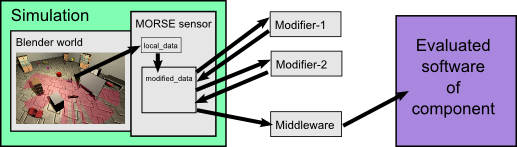
\includegraphics[width=500pt]{component_diagram.png}
\caption{Component data flow}
\end{figure*}

The data flow is similar for actuators, except that the direction is inversed, with the data arriving first from the evaluated software via the middleware, then processed by the modifiers and finally applied in the simulation.


\dokutitleleveltwo{Sensors}
\label{029aee483db9ae244d7a5cb353e74602}%% sensors

\begin{itemize}
\dokuitem  \hyperref[11648e4e66e7ed6a86cb7f1d0cf604fe]{ GPS}
\dokuitem  \hyperref[6b3b2d8500522343e080755f0e0aa4fe]{ Gyroscope}
\dokuitem  \hyperref[dd6d2dcc679d12b9430a9787bab45b33]{ Video camera}
\dokuitem  \hyperref[8d7d5ffd0031f2449cbeaef424c22d75]{ SICK laser}
\end{itemize}

\dokutitleleveltwo{Actuators/Controllers}
\label{2068e59180763f350d66a42e828e7f96}%% controllers

\begin{itemize}
\dokuitem  \hyperref[388a56dbb62a010dc26a378981346247]{ Keyboard arrows}
\dokuitem  \hyperref[cdf7afd8bc8dbb764b14c987cea8effd]{ Linear and angular speed (V, W)}
\dokuitem  \hyperref[6990a54322d9232390a784c5c9247dd6]{ Straight line movement}
\dokuitem  \hyperref[f75862c2bd0040eb683048c313dcaaa8]{ Waypoint destination}
\end{itemize}

\dokutitleleveltwo{Bare robotic bases}
\label{d69ac14cd721dd995822d4e984f48116}%% bare_robotic_bases

\begin{itemize}
\dokuitem  \hyperref[4fd87f5742582d412dce2c6ad5304937]{ iRobot ATRV}
\dokuitem  \hyperref[311954cf2f831f2289fb7fff75d15a7d]{ Yamaha RMax}
\dokuitem  \hyperref[3c16132d99703978dacd02b0808a4270]{ NeoBotix platform with PA-10 robotic arm}
\end{itemize}

\dokutitlelevelone{Middleware Support}
\label{4303941a1597ae94654bd96854480742}%% middleware_support
\label{9a05db9c4b60b0527010fd997682f523}%%Start: supported_middlewares => /home/slemaign/openrobots/data/pages/supported_middlewares.txt

Middlewares provide a means for the simulated data to be shared with external programs. MORSE is designed to be middleware independent, so that its internal functioning is not tied no any one particular middleware, but it is capable of communicating with any type of architecture.


\dokutitleleveltwo{Current list of compatible middlewares}
\label{92515de7e8c9f43d6ca122cbbfd1809e}%% current_list_of_compatible_middlewares

\begin{itemize}
\dokuitem  \hyperref[1cb251ec0d568de6a929b520c4aed8d1]{ Text file output}
\dokuitem  \hyperref[61f2529360aec54f5dc9804b842cf3fa]{ Sockets}
\dokuitem  \hyperref[ec46d0b85077d7a7fe8da2e2b4c70462]{ YARP}
\dokuitem  \hyperref[15f13a3fccdd1ef095539316b61c03c8]{ Pocolibs}
\end{itemize}

\dokutitleleveltwo{Linking a middleware in a scene}
\label{5ded332fc3ba470e4d4d290c9bf26a19}%% linking_a_middleware_in_a_scene

To be able to use a middleware inside of a scene, it is necessary to link the Empty object from the corresponding Blender file. This process is explained in the \hyperref[0575c8d592fb7b088226750aceec2b4e]{ basic tutorial} and the \hyperref[1dd029a60f7f3dd1deaf993ce4538edf]{ yarp tutorial}. Those pages also explain how to configure the components to use a given middleware.

Binding a component to use a middleware is done in the file \dokumonospace{component{\textunderscore}config.py} that should be part of every MORSE scenario file. In that file, the dictionary \dokumonospace{component{\textunderscore}mw} lists the components and the middleware they will use to export/import their data. The unique names of the components are the keys of the dictionary, and the values are lists. The first item in the list is the name of the middleware Empty object in the scene. The following items depend on the type of middleware, but will generally be the name of the middleware function that should be called by the component to share its data.


\dokutitleleveltwo{Expanding the middlewares}
\label{b3a6313d335453f4c7ad970485acc1a1}%% expanding_the_middlewares

New middlewares can be added to MORSE by following these \hyperref[6a8f80abb2f3d2288ad863e67f2499a4]{ instructions}.


\dokutitlelevelone{GPS sensor}
\label{fa7c7c892a3b7d9c01ef03ed367274b8}%% gps_sensor
\label{11648e4e66e7ed6a86cb7f1d0cf604fe}%%Start: gps => /home/slemaign/openrobots/data/pages/gps.txt

This sensor emulates a GPS, providing the exact coordinates in the Blender scene. The coordinates provided by the GPS are with respect to the origin of the Blender coordinate reference.


\dokutitleleveltwo{Files}
\label{45b963397aa40d4a0063e0d85e4fe7a1}%% files

\begin{itemize}
\dokuitem  Blender: \dokumonospace{{\textdollar}ORS{\textunderscore}ROOT/data/morse/components/sensors/morse{\textunderscore}GPS.blend}
\dokuitem  Python: \dokumonospace{{\textdollar}ORS{\textunderscore}ROOT/src/morse/sensors/gps.py}
\end{itemize}

\dokutitlelevelfour{Local data}

\begin{itemize}
\dokuitem  \dokubold{X}: X coordinate of the sensor
\dokuitem  \dokubold{Y}: Y coordinate of the sensor
\dokuitem  \dokubold{Z}: Z coordinate of the sensor
\end{itemize}

\dokuunderline{Note}: Coordinates are given with respect to the origin of Blender's coordinate axis.


\dokutitleleveltwo{Applicable modifiers}
\label{e70c0c8fd69fbf29dc4de09110825004}%% applicable_modifiers

This sensor always provides perfect data, with respect to an arbitrary point.
To obtain more realistic readings, it is recommended to add modifiers.
The two which are specially used for the GPS information are:



\begin{itemize}
\dokuitem  UTM modifier: Will add an offset to the Blender coordinates according to the parameters set on the scene.
\end{itemize}

\begin{itemize}
\dokuitem  NED: Changes the coordinate reference to use North (X), East (Y), Down (Z)
\end{itemize}

\begin{itemize}
\dokuitem  Noise modifier: Adds random Gaussian noise to the data
\end{itemize}

\dokutitlelevelone{Gyroscope sensor}
\label{85d7c1617c515754e4ff7f3604a0776f}%% gyroscope_sensor
\label{6b3b2d8500522343e080755f0e0aa4fe}%%Start: gyroscope => /home/slemaign/openrobots/data/pages/gyroscope.txt

This sensor emulates a Gyroscope, providing the yaw, pitch and roll angles of the sensor object with respect to the Blender world reference axes.
The angles are given in degrees.


\dokutitleleveltwo{Files}
\label{45b963397aa40d4a0063e0d85e4fe7a1}%% files

\begin{itemize}
\dokuitem  Blender: \dokumonospace{{\textdollar}ORS{\textunderscore}ROOT/data/morse/components/sensors/morse{\textunderscore}gyroscope.blend}
\dokuitem  Python: \dokumonospace{{\textdollar}ORS{\textunderscore}ROOT/src/morse/sensors/gyroscope.py}
\end{itemize}

\dokutitlelevelfour{Local data}

\begin{itemize}
\dokuitem  \dokubold{yaw}: rotation angle with respect to the Z axis
\dokuitem  \dokubold{pitch}: rotation angle with respect to the X axis
\dokuitem  \dokubold{roll}: rotation angle with respect to the Y axis
\end{itemize}

\dokuunderline{Note}: Coordinates are given with respect to the origin of Blender's coordinate axis.


\dokutitleleveltwo{Applicable modifiers}
\label{e70c0c8fd69fbf29dc4de09110825004}%% applicable_modifiers

This sensor always provides perfect data.
To obtain more realistic readings, it is recommended to add modifiers.



\begin{itemize}
\dokuitem  Noise modifier: Adds random Gaussian noise to the data
\end{itemize}

\dokutitleleveltwo{Related components}
\label{72610f0a0494668833b2c5de69dd5e02}%% related_components

Some other components of MORSE require a Gyroscope to be linked to the robot, in order to function properly. The \dokumonospace{Motion controller} actuator modules make use of the angles to instruct the robot to turn. If no Gyroscope is installed in the robot, the controllers will not work properly.


\dokutitlelevelone{Video camera sensor}
\label{2157f6689a9fa010e655f615edf5281d}%% video_camera_sensor
\label{dd6d2dcc679d12b9430a9787bab45b33}%%Start: camera => /home/slemaign/openrobots/data/pages/camera.txt

This sensor emulates a single video camera. It generates a series of RGBA images. Images are encoded as binary char arrays, with 4 bytes per pixel.

The cameras make use of Blender's \dokubold{VideoTexture} module, which requires a graphic card capable of GLSL shading. Also, the 3D view window in Blender must be set to draw \dokubold{Textured} objects.


\dokutitleleveltwo{Files}
\label{45b963397aa40d4a0063e0d85e4fe7a1}%% files

\begin{itemize}
\dokuitem  Blender: \dokumonospace{{\textdollar}ORS{\textunderscore}ROOT/data/morse/components/sensors/morse{\textunderscore}camera.blend}
\dokuitem  Python: \dokumonospace{{\textdollar}ORS{\textunderscore}ROOT/src/morse/sensors/camera.py}
\end{itemize}

\dokutitleleveltwo{Local data}
\label{a53af9dae307d714362321cf5d55d89c}%% local_data

\begin{itemize}
\dokuitem  \dokubold{image}: The data captured by the camera, stored as a binary string of size \dokumonospace{(\dokubold{cam{\textunderscore}width} X \dokubold{cam{\textunderscore}height} * 4)} bytes. The image is stored as RGBA.
\end{itemize}

\dokutitleleveltwo{Configurable parameters}
\label{576be46e2988ecd45f7341398c2cb015}%% configurable_parameters

The Empty object corresponding to this sensor has the following parameters:


\begin{itemize}
\dokuitem  \dokubold{capturing}: (Boolean) flag that determines whether the camera should generate an image. It can be toggled on or off by pressing the 'Spacebar'
\dokuitem  \dokubold{cam{\textunderscore}width}: (double) generated image width in pixels
\dokuitem  \dokubold{cam{\textunderscore}height}: (double) generated image height in pixels
\dokuitem  \dokubold{cam{\textunderscore}focal}: (double) camera focal length as defined in Blender (note: in Blender this parameter unit is "millimeters". This is actually misleading, as there is no dimension associated to Blender units.)
\end{itemize}

\dokutitleleveltwo{Camera calibration matrix}
\label{1ab5c786ae6eee706bb6b24a3298ccea}%% camera_calibration_matrix

The camera configuration parameters implicitly define a geometric camera in blender units. Knowing that the \dokubold{cam{\textunderscore}focal} attribute is a value that represents the distance in Blender unit at which the largest image dimension is 32.0 Blender units, the camera intrinsic calibration matrix is defined as:


%% Table analyse:
%%    Numrows: 3
%%    Longest row size: 25
%%    Choose table mode: tabular
\vspace{0.8em}
\begin{tabular}{llll}
\hline
\multicolumn{1}{|l|}{ \dokubold{alpha{\textunderscore}u} }&\multicolumn{1}{l|}{ 0 }&\multicolumn{1}{l|}{ \dokubold{u{\textunderscore}0} }&\multicolumn{1}{l|}{ 0 }\\ 
\hline
\multicolumn{1}{|l|}{ 0 }&\multicolumn{1}{l|}{ \dokubold{alpha{\textunderscore}v} }&\multicolumn{1}{l|}{ \dokubold{ v{\textunderscore}0} }&\multicolumn{1}{l|}{ 0 }\\ 
\hline
\multicolumn{1}{|l|}{ 0 }&\multicolumn{1}{l|}{ 0 }&\multicolumn{1}{l|}{ 1 }&\multicolumn{1}{l|}{ 0 }\\ 
\hline
\end{tabular}
\vspace{0.8em}


where:


\begin{itemize}
\dokuitem  \dokubold{alpha{\textunderscore}u} == \dokubold{ alpha{\textunderscore}v} = \dokubold{cam{\textunderscore}width} . \dokubold{cam{\textunderscore}focal} / 32 (we suppose here that \dokubold{cam{\textunderscore}width} $>$ \dokubold{cam{\textunderscore}height}. If not, then use \dokubold{cam{\textunderscore}height} in the formula)
\dokuitem  \dokubold{u{\textunderscore}0} = \dokubold{cam{\textunderscore}height} / 2
\dokuitem  \dokubold{v{\textunderscore}0} = \dokubold{cam{\textunderscore}width} / 2
\end{itemize}

\dokutitleleveltwo{Applicable modifiers}
\label{e70c0c8fd69fbf29dc4de09110825004}%% applicable_modifiers

No camera modifiers available at the moment


\dokutitleleveltwo{Related components}
\label{72610f0a0494668833b2c5de69dd5e02}%% related_components

A stereo bench is composed of two regular cameras (as described in this page) parented to a \hyperref[44100c7b616b78eac7bbbd83ad6e4786]{ pan-tilt unit}.


\dokutitlelevelone{SICK laser range scanner}
\label{95f36fb9159a6cb3d088ef15be471622}%% sick_laser_range_scanner
\label{8d7d5ffd0031f2449cbeaef424c22d75}%%Start: sick => /home/slemaign/openrobots/data/pages/sick.txt

This sensor emulates a laser range scanner, by generating a series of rays in predefined directions, and then computing whether they find any object within a certain distance of the sensor's origin.

\dokuunderline{Note}: Objects in the scene with the \dokubold{No collision} setting in their Game properties will not be detected by this sensor


\dokutitleleveltwo{Files}
\label{45b963397aa40d4a0063e0d85e4fe7a1}%% files

\begin{itemize}
\dokuitem  Blender: \dokumonospace{{\textdollar}ORS{\textunderscore}ROOT/data/morse/components/sensors/morse{\textunderscore}sick.blend}
\dokuitem  Python: \dokumonospace{{\textdollar}ORS{\textunderscore}ROOT/src/morse/sensors/sick.py}
\end{itemize}

\dokutitleleveltwo{Local data}
\label{a53af9dae307d714362321cf5d55d89c}%% local_data

\begin{itemize}
\dokuitem  \dokubold{point{\textunderscore}list}: Array that stores the positions of the points found by the laser. The points are given with respect to the location of the sensor, and stored as lists of three elements. The number of points depends on the geometry of the arc parented to the sensor (see below).
\end{itemize}

\dokutitleleveltwo{Configurable Parameters}
\label{576be46e2988ecd45f7341398c2cb015}%% configurable_parameters

The Empty object corresponding to this sensor has the following parameters:


\begin{itemize}
\dokuitem  \dokubold{Laser{\textunderscore}Range}: (double) The distance in meters from the center of the sensor to which it is capable of detecting other objects
\end{itemize}

  * \dokubold{Visible{\textunderscore}arc}: (Boolean) A toggle that determines whether the scanned area is displayed during the execution of the simulation or not. If the robot is also producing camera images, it is better to set this variable to False, otherwise the scanned area will also appear on the captured images.


\dokutitleleveltree{Number and angle of rays}
\label{0e26d09474e479fcb039d350438a39b6}%% number_and_angle_of_rays

The current way to configure the number of rays used by the SICK is to define a new object in the scene, a circle or semicircle with as many vertices as laser rays.
The easiest way to create the object in Blender is to \dokubold{Add{$\rightarrow$}Mesh{$\rightarrow$}Circle}. In the dialog that appears, give the number of vertices as necessary. Make sure to select the \dokubold{Fill} option, so that there will be a central vertex and the circle will have the faces already defined.

The new object must have the following characteristics:



\begin{itemize}
\dokuitem  Name: Its name must begin with 'Arc{\textunderscore}', for the SICK Module to recognize it. The currently used method is to name the arcs according to the number of rays they have, for example: Arc{\textunderscore}180, Arc{\textunderscore}16, Arc{\textunderscore}360
\end{itemize}

\begin{itemize}
\dokuitem  Vertices: It is necessary that the vertex at the center of the circle is at local coordinates 0, 0, 0. This is the default case, so it should not be modified.
\end{itemize}

\begin{itemize}
\dokuitem  Normals: For the circle to be visible in the GE, the normals of the faces must be facing up. Otherwise the object will not be displayed
\end{itemize}

\begin{itemize}
\dokuitem  Physics: Make sure that on the \dokubold{Logic Panel} this object is set to \dokubold{No collision}, otherwise it will push objects around
\end{itemize}

\dokutitlelevelone{Keyboard actuator}
\label{934862559c0fd0c289ad026052aa3842}%% keyboard_actuator
\label{388a56dbb62a010dc26a378981346247}%%Start: keyboard => /home/slemaign/openrobots/data/pages/keyboard.txt

This actuator does not require a connection with external data. It simply responds to the keyboard arrows to generate movement instructions for the robot attached.

When parented to a robot, the user can press the arrow keys to modify the linear and angular velocities (V, W) of the robot.


\begin{itemize}
\dokuitem  \key{{$\uparrow$}} forward
\dokuitem  \key{{$\downarrow$}} backwards
\dokuitem  \key{{$\leftarrow$}} turn left
\dokuitem  \key{{$\rightarrow$}} turn right
\end{itemize}

\dokutitleleveltwo{Files}
\label{45b963397aa40d4a0063e0d85e4fe7a1}%% files

\begin{itemize}
\dokuitem  Blender: \dokumonospace{{\textdollar}ORS{\textunderscore}ROOT/data/morse/components/controllers/morse{\textunderscore}manual{\textunderscore}control.blend}
\dokuitem  Python: \dokumonospace{{\textdollar}ORS{\textunderscore}ROOT/src/morse/actuators/keyboard.py}
\end{itemize}

\dokutitleleveltwo{Applicable modifiers}
\label{e70c0c8fd69fbf29dc4de09110825004}%% applicable_modifiers

No available modifiers


\dokutitlelevelone{Linear and angular speed (V, W) actuator}
\label{a5b03f17bedad4c5e66985756a9fc8af}%% linear_and_angular_speed_v_w_actuator
\label{cdf7afd8bc8dbb764b14c987cea8effd}%%Start: v_omega => /home/slemaign/openrobots/data/pages/v_omega.txt

This actuator reads the values of linear and angular speed and applies them to the robot. The speeds provided are internally adjusted to the Blender time measure.


\dokutitleleveltwo{Files}
\label{45b963397aa40d4a0063e0d85e4fe7a1}%% files

\begin{itemize}
\dokuitem  Blender: \dokumonospace{{\textdollar}ORS{\textunderscore}ROOT/data/morse/components/controllers/morse{\textunderscore}vw{\textunderscore}control.blend}
\dokuitem  Python: \dokumonospace{{\textdollar}ORS{\textunderscore}ROOT/src/morse/actuators/v{\textunderscore}omega.py}
\end{itemize}

\dokutitleleveltwo{Local data}
\label{a53af9dae307d714362321cf5d55d89c}%% local_data

\begin{itemize}
\dokuitem  \dokubold{v}: linear velocity
\dokuitem  \dokubold{w}: angular velocity
\end{itemize}

\dokutitleleveltwo{Applicable modifiers}
\label{e70c0c8fd69fbf29dc4de09110825004}%% applicable_modifiers

No available modifiers


\dokutitlelevelone{Straight line movement}
\label{90821a70309c40fdb782ed75db5c7b9a}%% straight_line_movement
\label{6990a54322d9232390a784c5c9247dd6}%%Start: destination => /home/slemaign/openrobots/data/pages/destination.txt

This actuator reads the coordinates of a destination point, and moves the robot in a straight line towards the given point, without turning.
It provides a very simplistic movement, and can be used for testing or for robots with holonomic movement.
The speeds provided are internally adjusted to the Blender time measure.


\dokutitleleveltwo{Files}
\label{45b963397aa40d4a0063e0d85e4fe7a1}%% files

\begin{itemize}
\dokuitem  Blender: \dokumonospace{{\textdollar}ORS{\textunderscore}ROOT/data/morse/components/controllers/morse{\textunderscore}destination{\textunderscore}control.blend}
\dokuitem  Python: \dokumonospace{{\textdollar}ORS{\textunderscore}ROOT/src/morse/actuators/destination.py}
\end{itemize}

\dokutitleleveltwo{Local data}
\label{a53af9dae307d714362321cf5d55d89c}%% local_data

\begin{itemize}
\dokuitem  \dokubold{x}: Destination X coordinate
\dokuitem  \dokubold{Y}: Destination Y coordinate
\dokuitem  \dokubold{Z}: Destination Z coordinate
\end{itemize}

\dokuunderline{Note}: Coordinates are given with respect to the origin of Blender's coordinate axis.


\dokutitleleveltwo{Applicable modifiers}
\label{e70c0c8fd69fbf29dc4de09110825004}%% applicable_modifiers

\begin{itemize}
\dokuitem  UTM modifier: Will add an offset to the Blender coordinates according to the parameters set on the scene.
\end{itemize}

\begin{itemize}
\dokuitem  NED: Changes the coordinate reference to use North (X), East (Y), Down (Z)
\end{itemize}

\dokutitlelevelone{Waypoint target movement}
\label{e333de84c053461b128b58be1929db98}%% waypoint_target_movement
\label{f75862c2bd0040eb683048c313dcaaa8}%%Start: waypoint => /home/slemaign/openrobots/data/pages/waypoint.txt

This actuator reads the coordinates of a destination point, and moves the robot towards the given point, with the robot restricted to moving only forward, backwards or turning over its Z axis.
This controller is meant to be used mainly by non-holonomic robots.
The speeds provided are internally adjusted to the Blender time measure.


\dokutitleleveltwo{Files}
\label{45b963397aa40d4a0063e0d85e4fe7a1}%% files

\begin{itemize}
\dokuitem  Blender: \dokumonospace{{\textdollar}ORS{\textunderscore}ROOT/data/morse/components/controllers/morse{\textunderscore}destination{\textunderscore}control.blend}
\dokuitem  Python: \dokumonospace{{\textdollar}ORS{\textunderscore}ROOT/src/morse/actuators/destination.py}
\end{itemize}

\dokutitleleveltree{Local data}
\label{a53af9dae307d714362321cf5d55d89c}%% local_data

\begin{itemize}
\dokuitem  \dokubold{x}: Destination X coordinate
\dokuitem  \dokubold{Y}: Destination Y coordinate
\dokuitem  \dokubold{Z}: Destination Z coordinate
\dokuitem  \dokubold{speed}: Movement speed
\end{itemize}

\dokuunderline{Note}: Coordinates are given with respect to the origin of Blender's coordinate axis.


\dokutitleleveltwo{Applicable modifiers}
\label{e70c0c8fd69fbf29dc4de09110825004}%% applicable_modifiers

\begin{itemize}
\dokuitem  UTM modifier: Will add an offset to the Blender coordinates according to the parameters set on the scene.
\end{itemize}

\begin{itemize}
\dokuitem  NED: Changes the coordinate reference to use North (X), East (Y), Down (Z)
\end{itemize}

\dokutitlelevelone{iRobot ATRV platform}
\label{51f82c2a17c65a05f749f4b5d80a19b3}%% irobot_atrv_platform
\label{4fd87f5742582d412dce2c6ad5304937}%%Start: atrv => /home/slemaign/openrobots/data/pages/atrv.txt

The base of the \dokubold{DALA} robot at LAAS.


\dokutitleleveltwo{Files}
\label{45b963397aa40d4a0063e0d85e4fe7a1}%% files

\begin{itemize}
\dokuitem  Blender: \dokumonospace{{\textdollar}ORS{\textunderscore}ROOT/data/morse/components/robots/atrv.blend}
\dokuitem  Python: \dokumonospace{{\textdollar}ORS{\textunderscore}ROOT/src/morse/robots/atrv.py}
\end{itemize}

\dokutitleleveltwo{Adjustable parameters}
\label{4997feebf90104aab2d79756367e9b42}%% adjustable_parameters

Use the Logic panel in Blender (shown with \key{F4}) to adjust the \dokubold{Mass} of the robot.


\dokutitlelevelone{Yamaha RMAX platform}
\label{997ffd08d6757c595f9c1d4ef5679d13}%% yamaha_rmax_platform
\label{311954cf2f831f2289fb7fff75d15a7d}%%Start: ressac => /home/slemaign/openrobots/data/pages/ressac.txt

The base of the \dokubold{Ressac} robot at ONERA.


\dokutitleleveltwo{Files}
\label{45b963397aa40d4a0063e0d85e4fe7a1}%% files

\begin{itemize}
\dokuitem  Blender: \dokumonospace{{\textdollar}ORS{\textunderscore}ROOT/data/morse/components/robots/ressac.blend}
\dokuitem  Python: \dokumonospace{{\textdollar}ORS{\textunderscore}ROOT/src/morse/robots/ressac.py}
\end{itemize}

\dokutitleleveltwo{Adjustable parameters}
\label{4997feebf90104aab2d79756367e9b42}%% adjustable_parameters

The rotation of the rotor is fixed and only for show. Its speed can be adjusted in the Logic panel in Blender (shown with \key{F4}) when the rotor object is selected.


\dokutitlelevelone{NeoBotix and PA-10 arm}
\label{1eef7a1b9401d909bf39e4ac86c3785a}%% neobotix_and_pa-10_arm
\label{3c16132d99703978dacd02b0808a4270}%%Start: jido => /home/slemaign/openrobots/data/pages/jido.txt

The base of the \dokubold{JIDO} robot at LAAS.


\dokutitleleveltwo{Files}
\label{45b963397aa40d4a0063e0d85e4fe7a1}%% files

\begin{itemize}
\dokuitem  Blender: \dokumonospace{{\textdollar}ORS{\textunderscore}ROOT/data/morse/components/robots/jido.blend}
\dokuitem  Python: \dokumonospace{{\textdollar}ORS{\textunderscore}ROOT/src/morse/robots/jido.py}
\end{itemize}

\dokutitleleveltwo{Adjustable parameters}
\label{4997feebf90104aab2d79756367e9b42}%% adjustable_parameters

The arm is rigged with an armature, following the mechanics of the arm. It is set to use Inverse Kinematics to follow an Empty object called \dokubold{Target{\textunderscore}Empty}. However, the IK solver is only available during execution of the simulation in Blender version 2.5 or higher. Thus, this remains as a future development.

%Rendering morse:user:modifier_introduction
\dokutitleleveltwo{Modifiers}
\label{bf24b44a8cc99e648657b164c8aba758}%% modifiers
\label{25bc6523e9298f4691b3c8200a395d92}%%Start: modifier_introduction => /home/slemaign/openrobots/data/pages/modifier_introduction.txt

Modifiers affect directly the data employed by sensors and actuators, and are specific to the data used by the components. Just like middlewares, they must implement a method called \dokumonospace{register{\textunderscore}component} that should add the corresponding function to the component's action list.


\dokutitleleveltwo{List of existing modifiers}
\label{e1bd7dc12fc91796f6afa908960bddfd}%% list_of_existing_modifiers

\begin{itemize}
\dokuitem  \hyperref[b32d6491ce03dd4e6c877f3bfd9ff07e]{ UTM conversion}
\dokuitem  \hyperref[f68daad189b2fffd0b8cab5e36ec9d96]{ NED conversion}
\dokuitem  \hyperref[466deec76ecdf5fca6d38571f6324d54]{ JSON encoding/decoding}
\dokuitem  \hyperref[aa061f2a51a69b41bf030cab71d64ed9]{ GPS noise}
\end{itemize}

\dokutitleleveltwo{Linking a modifier in a scene}
\label{840a8bd36b58f7e792398436a4be45db}%% linking_a_modifier_in_a_scene

To be able to use a modifier inside of a scene, it is necessary to link the Empty object from the corresponding Blender file. This process is identical to the one used for middlewares, as explained in the \hyperref[0575c8d592fb7b088226750aceec2b4e]{ basic tutorial}, together with an explanation on how to configure the components to call middleware functions.

Binding a component to use a modifier is done in the file \dokumonospace{component{\textunderscore}config.py} that should be part of every MORSE scenario file. In that file, the dictionary \dokumonospace{component{\textunderscore}modifier} lists the components and the modifiers they will use to export/import their data. The unique names of the components are the keys of the dictionary, and the values are lists. Each list will contain as many items as modifiers associated to the component, and each element is also a list. In these internal lists, the first element is the name of the modifier Empty object in the scene, and the second is the modifier method that should be called by the component to alter its data. Here is an example of the \dokumonospace{component{\textunderscore}modifier} dictionary:


\lstset{language=python}
\begin{lstlisting}
component_modifier = {
	"GPS": [ ["NED", "blender_to_ned"], ["UTM", "blender_to_utm"] ],
	"Motion_Controller": [ ["NED", "ned_to_blender"], ["UTM", "utm_to_blender"] ],
	"Thermometer": [ ["Json", "json_encode"] ],
	}

\end{lstlisting}

\dokutitleleveltwo{Creating a new modifier}
\label{2f5deef38336990fa7f864f2028d68a9}%% creating_a_new_modifier

The concept of a modifier is relatively simple. Their only function is to change the data stored in variables in the corresponding component, by using the concept of \hyperref[4e819c837d54a6ed09abc77a8560a66f]{hooks}. Creating a new modifier consists mainly of writing the Python script that will alter the data. The modifier should only work on the \dokumonospace{modified{\textunderscore}data} array of a MORSE component, and it is important to ensure the fields of the array are maintained with the same order and data type.


\dokutitlelevelone{UTM conversion}
\label{df94310d1616e05688abb99eb76758dc}%% utm_conversion
\label{b32d6491ce03dd4e6c877f3bfd9ff07e}%%Start: utm => /home/slemaign/openrobots/data/pages/utm.txt
This modifier converts the coordinates generated by the MORSE simulator to use UTM global coordinates. This is achieved by setting the offset of the Blender origin with respect to the UTM reference. The offset is stored as three properties of the \dokumonospace{Scene{\textunderscore}Script{\textunderscore}Holder} object of the scene: \dokumonospace{UTMXOffset}, \dokumonospace{UTMYOffset} and \dokumonospace{UTMZOffset}.


\dokutitleleveltwo{Files}
\label{45b963397aa40d4a0063e0d85e4fe7a1}%% files

\begin{itemize}
\dokuitem  Blender: \dokumonospace{{\textdollar}ORS{\textunderscore}ROOT/data/morse/components/modifiers/utm{\textunderscore}empty.blend}
\dokuitem  Python: \dokumonospace{{\textdollar}ORS{\textunderscore}ROOT/src/morse/modifiers/utm{\textunderscore}mod.py}
\end{itemize}

\dokutitleleveltree{Modified data}
\label{c1a1a093b7ca2545d0d88cac0ff8ccf6}%% modified_data
Modifiers work over an array called \dokumonospace{modified{\textunderscore}data} of the components.
The indices of the variables affected are the following:


\begin{itemize}
\dokuitem  \dokubold{0}: X coordinate of the component
\dokuitem  \dokubold{1}: Y coordinate of the component
\dokuitem  \dokubold{2}: Z coordinate of the component
\end{itemize}

For example, changing the X coordinate is done by altering the value of \dokumonospace{modified{\textunderscore}data[0]}.


\dokutitleleveltwo{Available methods}
\label{a2d06dcb42bbd0519b19166fd7f36cea}%% available_methods

\begin{itemize}
\dokuitem  \dokumonospace{blender{\textunderscore}to{\textunderscore}utm}: Used for the \hyperref[11648e4e66e7ed6a86cb7f1d0cf604fe]{ GPS sensor}
\dokuitem  \dokumonospace{utm{\textunderscore}to{\textunderscore}blender}: Used for the \hyperref[6990a54322d9232390a784c5c9247dd6]{ Straight} and \hyperref[f75862c2bd0040eb683048c313dcaaa8]{ Waypoint} actuators
\end{itemize}

\dokutitlelevelone{NED conversion}
\label{95cc2c00e60ea8d7ee8c566b6598de36}%% ned_conversion
\label{f68daad189b2fffd0b8cab5e36ec9d96}%%Start: ned => /home/slemaign/openrobots/data/pages/ned.txt
This modifier converts the coordinates generated by the MORSE simulator to change to the North, East, Down (NED) coordinate system, instead of the East, North, Up (ENU) system normally used by Blender.
This is achieved by switching the direction of the X and Y axis, as well as inverting the sense of the Z axis.


\dokutitleleveltwo{Files}
\label{45b963397aa40d4a0063e0d85e4fe7a1}%% files

\begin{itemize}
\dokuitem  Blender: \dokumonospace{{\textdollar}ORS{\textunderscore}ROOT/data/morse/components/modifiers/ned{\textunderscore}empty.blend}
\dokuitem  Python: \dokumonospace{{\textdollar}ORS{\textunderscore}ROOT/src/morse/modifiers/ned{\textunderscore}mod.py}
\end{itemize}

\dokutitleleveltree{Modified data}
\label{c1a1a093b7ca2545d0d88cac0ff8ccf6}%% modified_data
Modifiers work over an array called \dokumonospace{modified{\textunderscore}data} of the components.
The indices of the variables affected are the following:


\begin{itemize}
\dokuitem  \dokubold{0}: X coordinate of the component
\dokuitem  \dokubold{1}: Y coordinate of the component
\dokuitem  \dokubold{2}: Z coordinate of the component
\end{itemize}

For example, changing the X coordinate is done by altering the value of \dokumonospace{modified{\textunderscore}data[0]}.


\dokutitleleveltwo{Available methods}
\label{a2d06dcb42bbd0519b19166fd7f36cea}%% available_methods

\begin{itemize}
\dokuitem  \dokumonospace{blender{\textunderscore}to{\textunderscore}ned}: Used for the \hyperref[11648e4e66e7ed6a86cb7f1d0cf604fe]{ GPS sensor}
\dokuitem  \dokumonospace{ned{\textunderscore}to{\textunderscore}blender}: Used for the \hyperref[6990a54322d9232390a784c5c9247dd6]{ Straight} and \hyperref[f75862c2bd0040eb683048c313dcaaa8]{ Waypoint} actuators
\end{itemize}

\dokutitlelevelone{JSON encoding}
\label{2e3b13382733d486a7c0529f6a875385}%% json_encoding
\label{466deec76ecdf5fca6d38571f6324d54}%%Start: json => /home/slemaign/openrobots/data/pages/json.txt
This modifier transforms the \dokumonospace{modified{\textunderscore}data} array to contain a single item, which is a string with the data encoded using JSON.


\dokutitleleveltwo{Files}
\label{45b963397aa40d4a0063e0d85e4fe7a1}%% files

\begin{itemize}
\dokuitem  Blender: \dokumonospace{{\textdollar}ORS{\textunderscore}ROOT/data/morse/components/modifiers/json{\textunderscore}empty.blend}
\dokuitem  Python: \dokumonospace{{\textdollar}ORS{\textunderscore}ROOT/src/morse/modifiers/json{\textunderscore}mod.py}
\end{itemize}

\dokutitleleveltree{Modified data}
\label{c1a1a093b7ca2545d0d88cac0ff8ccf6}%% modified_data
This modifier replaces the whole \dokumonospace{modified{\textunderscore}data} array, switching however many items it has for a single one of type string.


\dokutitleleveltwo{Available methods}
\label{a2d06dcb42bbd0519b19166fd7f36cea}%% available_methods

\begin{itemize}
\dokuitem  \dokumonospace{json{\textunderscore}encode}: Change the data into a string
\dokuitem  \dokumonospace{json{\textunderscore}decode}: Expand the string into an array
\end{itemize}

\dokutitlelevelone{Tutorial example}
\label{d0e1bed8b40ec8e4f9cc0cc0a11ff110}%% tutorial_example
\label{0575c8d592fb7b088226750aceec2b4e}%%Start: tutorial => /home/slemaign/openrobots/data/pages/tutorial.txt

This tutorial assumes MORSE is properly installed. If not, follow the instructions \hyperref[ea09bb364ef1bffd889e76b7a59035fc]{ here}.


\dokutitleleveltwo{Setup of the simulation scene}
\label{80527725485ea9e7bedbc9d918895a02}%% setup_of_the_simulation_scene

\dokutitleleveltree{Load sample file}
\label{4238ab1e3d8f80f2fdec7f34e17e0f67}%% load_sample_file

Open the MORSE simulator with the test file provided with the installation, by using this command:



\small
\begin{verbatimtab}
$ morse $ORS_ROOT/share/morse/examples/scenarii/example-1.blend
\end{verbatimtab}
\normalsize

This will load a scene with a robot in a room with some furniture.


\dokutitleleveltree{Link an actuator}
\label{81c6b973417d3e5000d27d9c1c805b96}%% link_an_actuator

We'll add a motion controller to the robot, so that it can receive commands from an external program. The robot will then move according to the instructions received. In this case we'll add a controller that uses linear and angular speed (V, W).



\begin{enumerate}\dokuitem  With the mouse over the 3D view in Blender, press \key{Shift + F1} to open the Load Library browser
\dokuitem  Navigate to the directory \dokumonospace{{\textdollar}ORS{\textunderscore}ROOT/data/morse/components/controllers}
\dokuitem  Press 
\includegraphics[height=1em]{LMB.png} over the file \dokumonospace{morse{\textunderscore}vw{\textunderscore}control.blend}
\dokuitem  Press 
\includegraphics[height=1em]{LMB.png} over the item \dokumonospace{Object}
\dokuitem  Toggle the buttons \dokubold{Relative Paths} and \dokubold{Link} at the bottom of the window
\dokuitem  Press 
\includegraphics[height=1em]{RMB.png} over the item \dokumonospace{Motion{\textunderscore}Controller}
\dokuitem  Press the button \dokubold{Load Library}. You'll return to the 3D View
\dokuitem  Select the newly inserted object in the scene, either by 
\includegraphics[height=1em]{RMB.png} clicking over the object in the 3D View, or 
\includegraphics[height=1em]{LMB.png} over the object's name in the Outliner window. The object will be highlighted in cyan color, and can not be moved around.
\dokuitem  Convert the object to local, by pressing \key{L} then hitting \key{Enter}
\dokuitem  With the controller selected, hold down \key{Shift} and then 
\includegraphics[height=1em]{RMB.png} over the robot object
\dokuitem  Press \key{Ctrl + P} and then hit \key{Enter} make the robot the parent of the controller
\end{enumerate}

\dokutitleleveltree{Link a Gyroscope sensor}
\label{f019fe80659ff060e77872347a3add5c}%% link_a_gyroscope_sensor

Next we'll add a sensor to the robot that will report the angles of the robot orientation with respect to the reference axes (yaw, pitch and roll)



\begin{enumerate}\dokuitem  With the mouse over the 3D view in Blender, press \key{Shift + F1} to open the Load Library browser
\dokuitem  Navigate to the directory \dokumonospace{{\textdollar}ORS{\textunderscore}ROOT/data/morse/components/sensors}
\dokuitem  Press 
\includegraphics[height=1em]{LMB.png} over the file \dokumonospace{morse{\textunderscore}gyroscope.blend}
\dokuitem  Press 
\includegraphics[height=1em]{LMB.png} over the item \dokumonospace{Object}
\dokuitem  Toggle the buttons \dokubold{Relative Paths} and \dokubold{Link} at the bottom of the window
\dokuitem  Press 
\includegraphics[height=1em]{RMB.png} over the items \dokumonospace{Gyroscope} and \dokumonospace{Gyro{\textunderscore}box}
\dokuitem  Press the button \dokubold{Load Library}. You'll return to the 3D View
\dokuitem  Select the newly inserted \dokumonospace{Gyroscope} object in the scene, either by 
\includegraphics[height=1em]{RMB.png} clicking over the object in the 3D View, or 
\includegraphics[height=1em]{LMB.png} over the object's name in the Outliner window. The object will be highlighted in cyan color, and can not be moved around.
\dokuitem  Select the child object, by pressing \key{Shift + G}, then hitting \key{Enter}
\dokuitem  Convert the object to local, by pressing \key{L} then hitting \key{Enter}
\dokuitem  Switch to front view by pressing \key{'1 NumPad'}
\dokuitem  Press \key{G}, then move the \dokumonospace{Gyroscope} object to the correct location with respect to the robot
\dokuitem  Press 
\includegraphics[height=1em]{LMB.png} to accept the movement
\dokuitem  With the \dokumonospace{Gyroscope} object selected, hold down \key{Shift} and then 
\includegraphics[height=1em]{RMB.png} over the robot object
\dokuitem  Press \key{Ctrl + P} and then hit \key{Enter} make the robot the parent of the controller
\end{enumerate}

\dokutitleleveltree{Insert the middleware object}
\label{fc2213e90f6f9853c66c14f9f79c3379}%% insert_the_middleware_object
To use a middleware to exchange data from the simulator, it is necessary to link in an object that will represent the middleware.



\begin{enumerate}\dokuitem  With the mouse over the 3D view in Blender, press \key{Shift + F1} to open the Load Library browser
\dokuitem  Navigate to the directory \dokumonospace{{\textdollar}ORS{\textunderscore}ROOT/data/morse/components/middleware}
\dokuitem  Press 
\includegraphics[height=1em]{LMB.png} over the file \dokumonospace{socket{\textunderscore}empty.blend}
\dokuitem  Press 
\includegraphics[height=1em]{LMB.png} over the item \dokumonospace{Object}
\dokuitem  Toggle the buttons \dokubold{Relative Paths} and \dokubold{Link} at the bottom of the window
\dokuitem  Press 
\includegraphics[height=1em]{RMB.png} over the item \dokumonospace{Socket{\textunderscore}Empty}
\dokuitem  Press the button \dokubold{Load Library}. You'll return to the 3D View
\dokuitem  It is not necessary to make this object local or to move it. But it can be useful to avoid cluttering of items in the scene
\end{enumerate}

\dokuunderline{Note}: One single middleware Empty is necessary to enable the middleware, regardless of how many components will make use of it.


\dokutitleleveltree{Configuring the middlewares}
\label{7c1b9786b6402b908e3042548cd3c1c6}%% configuring_the_middlewares
Binding the components in the scene with the middleware is done in a configuration file within the Blender file.



\begin{enumerate}\dokuitem  On the \dokubold{Text Editor} window, select the file \dokumonospace{component{\textunderscore}config.py}
\dokuitem  Add the following items to the \dokumonospace{component{\textunderscore}mw} dictionary:
\end{enumerate}

\lstset{language=python}
\begin{lstlisting}
component_mw = {
    "Gyroscope": ["Socket", "post_message"],
    "Motion_Controller": ["Socket", "read_message"],
	}

\end{lstlisting}

\dokutitleleveltree{Run the simulation}
\label{62874528899bc63c891e142b192d89b7}%% run_the_simulation
Press \key{P} to start the Game Engine


\dokutitleleveltree{Connect with the client}
\label{646d760bcdaf8445e5fb3dbad2c443e5}%% connect_with_the_client
Use the example client program to test the bindings in the simulation



\begin{enumerate}\dokuitem  On a separate terminal, navigate to the directory \dokumonospace{{\textdollar}ORS{\textunderscore}ROOT/share/morse/examples/clients/atrv/}
\dokuitem  Execute the command
\end{enumerate}
    {\textdollar} python socket{\textunderscore}v{\textunderscore}omega{\textunderscore}client.py


\begin{enumerate}\dokuitem  Press \key{A} to give speed commands to the robot
\dokuitem  Type a the linear and angular speeds, followed by \key{Enter} after each
\dokuitem  The robot should start moving in MORSE
\dokuitem  Press \key{B} to print the readings of the gyroscope exported by MORSE
\dokuitem  Press \key{Q} to exit the client
\end{enumerate}

Finally exit the simulation, by pressing \key{Esc} on the Blender window, then close Blender by pressing \key{Ctrl + Q}, then \key{Enter}.


\dokutitlelevelone{Component bindings with middlewares (hooks)}
\label{af01c0ab3913f320e049366e6563bad8}%% component_bindings_with_middlewares_hooks
\label{4e819c837d54a6ed09abc77a8560a66f}%%Start: hooks => /home/slemaign/openrobots/data/pages/hooks.txt

\dokutitleleveltwo{Description of hooks}
\label{8d7cc6aa2e934c4272afb1f3080c4ad7}%% description_of_hooks

MORSE sensors and actuators are completely independent of any middleware,
and do not include themselves any means of passing the data they use.
To be able to use this data outside the simulator, it is necessary to bind
a middleware to every component, specifying the expected behavior.

When a component is linked to a middleware, a function described in the middleware will be added to the list of methods executed by the component, to be called each time the component executes its main task. In this way, the middleware can read the data provided by the component via a "hook", which is an established data structure.

MORSE components have a property called \dokumonospace{modified{\textunderscore}data}. It is a list that contains the data that can be exchanged with external programs. They also have a dictionary called \dokumonospace{local{\textunderscore}data} that has the names of the variables as well as their values, and is reserved for internal use in the component. Middlewares create the "hooks" to \dokumonospace{modified{\textunderscore}data} only.

Data modifiers can also be applied to the \dokumonospace{modified{\textunderscore}data} array, to produce data that is more realistic. In the case of sensors, the modifiers are applied before the data is sent through the middleware. The opposite happens with actuators, which read data through middlewares and then change it using modifiers, before using it inside of Blender.


\dokutitleleveltwo{Configuration}
\label{ccd1066343c95877b75b79d47c36bebe}%% configuration

This binding is currently done via a Python file called \dokumonospace{component{\textunderscore}config.py}
which must be internal to the Blender scenario file. The configuration file should be edited from a \dokubold{Text Editor} window in Blender.
It consists of two dictionaries indexed by the name of the components:

* \dokumonospace{component{\textunderscore}mw}: Lists which middlewares are bound to the specific component. The value of the dictionary is a list. The first element of the list is the name of the Middleware, and must be written exactly as the name of the Empty object that represents the Middleware in the scene.
In the case of Yarp and Text, the second item will be the name of the function to be added to the component's action list For Pocolibs, the second item is the type of poster, and the third is the name of the poster.

* \dokumonospace{component{\textunderscore}modifier}: Lists the modifiers affecting each of the components. The value of the dictionary is a list, where each element is itself a list representing a modifier. Each modifier list has two elements: the name of the modifier and the name of the function to use.

Example:


\lstset{language=python}
\begin{lstlisting}
component_mw = {
	Gyroscope": ["Yarp", "post_message"],
	"Motion_Controller": ["Yarp", "read_message"],
	"Motion_Controller.001": ["Pocolibs", "genPos", "p3dSpeedRef"],
	"CameraMain": ["Yarp", "post_image_RGBA"]
		}

component_modifier = {
	"GPS.001": [ ["NED", "blender_to_ned"], ["Json", "json_encode"] ],
	"Motion_Controller": [ ["NED", "ned_to_blender"] ],
		}

\end{lstlisting}
%Rendering morse:user:supported_middlewares
\dokutitlelevelone{Middleware Support}
\label{4303941a1597ae94654bd96854480742}%% middleware_support
\label{9a05db9c4b60b0527010fd997682f523}%%Start: supported_middlewares => /home/slemaign/openrobots/data/pages/supported_middlewares.txt

Middlewares provide a means for the simulated data to be shared with external programs. MORSE is designed to be middleware independent, so that its internal functioning is not tied no any one particular middleware, but it is capable of communicating with any type of architecture.


\dokutitleleveltwo{Current list of compatible middlewares}
\label{92515de7e8c9f43d6ca122cbbfd1809e}%% current_list_of_compatible_middlewares

\begin{itemize}
\dokuitem  \hyperref[1cb251ec0d568de6a929b520c4aed8d1]{ Text file output}
\dokuitem  \hyperref[61f2529360aec54f5dc9804b842cf3fa]{ Sockets}
\dokuitem  \hyperref[ec46d0b85077d7a7fe8da2e2b4c70462]{ YARP}
\dokuitem  \hyperref[15f13a3fccdd1ef095539316b61c03c8]{ Pocolibs}
\end{itemize}

\dokutitleleveltwo{Linking a middleware in a scene}
\label{5ded332fc3ba470e4d4d290c9bf26a19}%% linking_a_middleware_in_a_scene

To be able to use a middleware inside of a scene, it is necessary to link the Empty object from the corresponding Blender file. This process is explained in the \hyperref[0575c8d592fb7b088226750aceec2b4e]{ basic tutorial} and the \hyperref[1dd029a60f7f3dd1deaf993ce4538edf]{ yarp tutorial}. Those pages also explain how to configure the components to use a given middleware.

Binding a component to use a middleware is done in the file \dokumonospace{component{\textunderscore}config.py} that should be part of every MORSE scenario file. In that file, the dictionary \dokumonospace{component{\textunderscore}mw} lists the components and the middleware they will use to export/import their data. The unique names of the components are the keys of the dictionary, and the values are lists. The first item in the list is the name of the middleware Empty object in the scene. The following items depend on the type of middleware, but will generally be the name of the middleware function that should be called by the component to share its data.


\dokutitleleveltwo{Expanding the middlewares}
\label{b3a6313d335453f4c7ad970485acc1a1}%% expanding_the_middlewares

New middlewares can be added to MORSE by following these \hyperref[6a8f80abb2f3d2288ad863e67f2499a4]{ instructions}.


\dokutitlelevelone{Text middleware}
\label{f95f886458814bea9965b5a85aedb74b}%% text_middleware
\label{1cb251ec0d568de6a929b520c4aed8d1}%%Start: text => /home/slemaign/openrobots/data/pages/text.txt
This is the simplest method to export information from MORSE. The data gathered by components configured to use this "middleware" will be stored in simple text files. Currently this middleware is only used to output information, so it is only available for sensors.

File names used in MORSE have the following format: \dokumonospace{[robot{\textunderscore}name]{\textunderscore}[component{\textunderscore}name].txt}. Each file will have a header stating the name of the robot and the sensor, as well as the position of the sensor with respect to the center of the robot. The position is given with the format:


\lstset{language=python}
\begin{lstlisting}
(distance, globalVector(3), localVector(3))

\end{lstlisting}
Where \dokumonospace{globalVector} is a list of 3 elements with the X, Y and Z coordinates of the sensor with respect to the global origin. \dokumonospace{localVector} gives the coordinates with respect to the position of the robot.


\dokutitleleveltwo{Files}
\label{45b963397aa40d4a0063e0d85e4fe7a1}%% files

\begin{itemize}
\dokuitem  Blender: \dokumonospace{{\textdollar}ORS{\textunderscore}ROOT/data/morse/components/middleware/text{\textunderscore}empty.blend}
\dokuitem  Python: \dokumonospace{{\textdollar}ORS{\textunderscore}ROOT/src/morse/modifiers/text{\textunderscore}mw.py}
\end{itemize}

\dokutitleleveltwo{Available methods}
\label{a2d06dcb42bbd0519b19166fd7f36cea}%% available_methods

\begin{itemize}
\dokuitem  \dokumonospace{write{\textunderscore}data}: It will print to the file the current position of the robot, at the time of the sensor reading, followed by the list of variables in \dokumonospace{data{\textunderscore}keys} and the values in \dokumonospace{modified{\textunderscore}data}.
\end{itemize}

\dokutitlelevelone{Sockets}
\label{ffe33a3f6e35505faba01d17fd07d641}%% sockets
\label{61f2529360aec54f5dc9804b842cf3fa}%%Start: socket => /home/slemaign/openrobots/data/pages/socket.txt
A simple method to export data through the network. The MORSE sockets middleware will create a single UDP port for each robot, and the communication for all components of the robot using sockets will be made through the same port.
Data is shared as simple text strings.

\dokuunderline{Note}: The port numbers used in MORSE start at 70000.


\dokutitleleveltwo{Files}
\label{45b963397aa40d4a0063e0d85e4fe7a1}%% files

\begin{itemize}
\dokuitem  Blender: \dokumonospace{{\textdollar}ORS{\textunderscore}ROOT/data/morse/components/middleware/socket{\textunderscore}empty.blend}
\dokuitem  Python: \dokumonospace{{\textdollar}ORS{\textunderscore}ROOT/src/morse/modifiers/socket{\textunderscore}mw.py}
\end{itemize}

\dokutitleleveltwo{Available methods}
\label{a2d06dcb42bbd0519b19166fd7f36cea}%% available_methods

\begin{itemize}
\dokuitem  \dokumonospace{read{\textunderscore}message}: Gets information from a port, and stores it in the \dokumonospace{modified{\textunderscore}data} array of the associated component. This method expects a list of variables.
\dokuitem  \dokumonospace{post{\textunderscore}message}: Formats the contents of \dokumonospace{modified{\textunderscore}data} into a string separated by ';', and sends it through the port associated with a component. This method is only able to handle data of types: integer, float and string.
\end{itemize}

\dokutitlelevelone{YARP}
\label{ec46d0b85077d7a7fe8da2e2b4c70462}%% yarp
\label{ec46d0b85077d7a7fe8da2e2b4c70462}%%Start: yarp => /home/slemaign/openrobots/data/pages/yarp.txt
The YARP middleware provides a simple method to share data across components in different computers. It is based on the concept of \dokuitalic{ports}, which are registered in a \dokuitalic{name server} to differentiate between separate channels of communication.
Data is shared in the format of bottles, which are nested data structures of various data types.

\dokuunderline{Note}: Port names used in MORSE have the following format:\\ \dokumonospace{/ors/robots/[robot{\textunderscore}name]/[component{\textunderscore}name]/[direction]}. The term [direction] is either \dokumonospace{in} or \dokumonospace{out}, depending on the type of component being actuator or sensor, respectively.


\dokutitleleveltwo{Files}
\label{45b963397aa40d4a0063e0d85e4fe7a1}%% files

\begin{itemize}
\dokuitem  Blender: \dokumonospace{{\textdollar}ORS{\textunderscore}ROOT/data/morse/components/middleware/yarp{\textunderscore}empty.blend}
\dokuitem  Python: \dokumonospace{{\textdollar}ORS{\textunderscore}ROOT/src/morse/modifiers/yarp{\textunderscore}mw.py}
\end{itemize}

\dokutitleleveltwo{Available methods}
\label{a2d06dcb42bbd0519b19166fd7f36cea}%% available_methods

\begin{itemize}
\dokuitem  \dokumonospace{read{\textunderscore}message}: Gets information from a port, and stores it in the \dokumonospace{modified{\textunderscore}data} array of the associated component. This method is only able to handle data of types: integer, float and string.
\dokuitem  \dokumonospace{post{\textunderscore}message}: Formats the contents of \dokumonospace{modified{\textunderscore}data} into a bottle, and sends it through the port associated with a component. This method is only able to handle data of types: integer, float and string.
\dokuitem  \dokumonospace{post{\textunderscore}image{\textunderscore}RGBA}: (Requires YARP version 2.5+) Sends an image through a specialised port. The image must be stored in \dokumonospace{modified{\textunderscore}data} as a binary string with 32bit pixels encoded as RGBA. The actual size of the image is read directly from the component instance that called this method.
\end{itemize}

\dokutitlelevelone{Tutorial example}
\label{d0e1bed8b40ec8e4f9cc0cc0a11ff110}%% tutorial_example
\label{0575c8d592fb7b088226750aceec2b4e}%%Start: tutorial => /home/slemaign/openrobots/data/pages/tutorial.txt

This tutorial assumes MORSE is properly installed. If not, follow the instructions \hyperref[ea09bb364ef1bffd889e76b7a59035fc]{ here}.


\dokutitleleveltwo{Setup of the simulation scene}
\label{80527725485ea9e7bedbc9d918895a02}%% setup_of_the_simulation_scene

\dokutitleleveltree{Load sample file}
\label{4238ab1e3d8f80f2fdec7f34e17e0f67}%% load_sample_file

Open the MORSE simulator with the test file provided with the installation, by using this command:



\small
\begin{verbatimtab}
$ morse $ORS_ROOT/share/morse/examples/scenarii/example-1.blend
\end{verbatimtab}
\normalsize

This will load a scene with a robot in a room with some furniture.


\dokutitleleveltree{Link an actuator}
\label{81c6b973417d3e5000d27d9c1c805b96}%% link_an_actuator

We'll add a motion controller to the robot, so that it can receive commands from an external program. The robot will then move according to the instructions received. In this case we'll add a controller that uses linear and angular speed (V, W).



\begin{enumerate}\dokuitem  With the mouse over the 3D view in Blender, press \key{Shift + F1} to open the Load Library browser
\dokuitem  Navigate to the directory \dokumonospace{{\textdollar}ORS{\textunderscore}ROOT/data/morse/components/controllers}
\dokuitem  Press 
\includegraphics[height=1em]{LMB.png} over the file \dokumonospace{morse{\textunderscore}vw{\textunderscore}control.blend}
\dokuitem  Press 
\includegraphics[height=1em]{LMB.png} over the item \dokumonospace{Object}
\dokuitem  Toggle the buttons \dokubold{Relative Paths} and \dokubold{Link} at the bottom of the window
\dokuitem  Press \includegraphics[height=1em]{RMB.png} over the item \dokumonospace{Motion{\textunderscore}Controller}
\dokuitem  Press the button \dokubold{Load Library}. You'll return to the 3D View
\dokuitem  Select the newly inserted object in the scene, either by \includegraphics[height=1em]{RMB.png} clicking over the object in the 3D View, or \includegraphics[height=1em]{LMB.png} over the object's name in the Outliner window. The object will be highlighted in cyan color, and can not be moved around.
\dokuitem  Convert the object to local, by pressing \key{L} then hitting \key{Enter}
\dokuitem  With the controller selected, hold down \key{Shift} and then \includegraphics[height=1em]{RMB.png} over the robot object
\dokuitem  Press \key{Ctrl + P} and then hit \key{Enter} make the robot the parent of the controller
\end{enumerate}

\dokutitleleveltree{Link a Gyroscope sensor}
\label{f019fe80659ff060e77872347a3add5c}%% link_a_gyroscope_sensor

Next we'll add a sensor to the robot that will report the angles of the robot orientation with respect to the reference axes (yaw, pitch and roll)



\begin{enumerate}\dokuitem  With the mouse over the 3D view in Blender, press \key{Shift + F1} to open the Load Library browser
\dokuitem  Navigate to the directory \dokumonospace{{\textdollar}ORS{\textunderscore}ROOT/data/morse/components/sensors}
\dokuitem  Press \includegraphics[height=1em]{LMB.png} over the file \dokumonospace{morse{\textunderscore}gyroscope.blend}
\dokuitem  Press \includegraphics[height=1em]{LMB.png} over the item \dokumonospace{Object}
\dokuitem  Toggle the buttons \dokubold{Relative Paths} and \dokubold{Link} at the bottom of the window
\dokuitem  Press \includegraphics[height=1em]{RMB.png} over the items \dokumonospace{Gyroscope} and \dokumonospace{Gyro{\textunderscore}box}
\dokuitem  Press the button \dokubold{Load Library}. You'll return to the 3D View
\dokuitem  Select the newly inserted \dokumonospace{Gyroscope} object in the scene, either by \includegraphics[height=1em]{RMB.png} clicking over the object in the 3D View, or \includegraphics[height=1em]{LMB.png} over the object's name in the Outliner window. The object will be highlighted in cyan color, and can not be moved around.
\dokuitem  Select the child object, by pressing \key{Shift + G}, then hitting \key{Enter}
\dokuitem  Convert the object to local, by pressing \key{L} then hitting \key{Enter}
\dokuitem  Switch to front view by pressing \key{'1 NumPad'}
\dokuitem  Press \key{G}, then move the \dokumonospace{Gyroscope} object to the correct location with respect to the robot
\dokuitem  Press \includegraphics[height=1em]{LMB.png} to accept the movement
\dokuitem  With the \dokumonospace{Gyroscope} object selected, hold down \key{Shift} and then \includegraphics[height=1em]{RMB.png} over the robot object
\dokuitem  Press \key{Ctrl + P} and then hit \key{Enter} make the robot the parent of the controller
\end{enumerate}

\dokutitleleveltree{Insert the middleware object}
\label{fc2213e90f6f9853c66c14f9f79c3379}%% insert_the_middleware_object
To use a middleware to exchange data from the simulator, it is necessary to link in an object that will represent the middleware.



\begin{enumerate}\dokuitem  With the mouse over the 3D view in Blender, press \key{Shift + F1} to open the Load Library browser
\dokuitem  Navigate to the directory \dokumonospace{{\textdollar}ORS{\textunderscore}ROOT/data/morse/components/middleware}
\dokuitem  Press \includegraphics[height=1em]{LMB.png} over the file \dokumonospace{socket{\textunderscore}empty.blend}
\dokuitem  Press \includegraphics[height=1em]{LMB.png} over the item \dokumonospace{Object}
\dokuitem  Toggle the buttons \dokubold{Relative Paths} and \dokubold{Link} at the bottom of the window
\dokuitem  Press \includegraphics[height=1em]{RMB.png} over the item \dokumonospace{Socket{\textunderscore}Empty}
\dokuitem  Press the button \dokubold{Load Library}. You'll return to the 3D View
\dokuitem  It is not necessary to make this object local or to move it. But it can be useful to avoid cluttering of items in the scene
\end{enumerate}

\dokuunderline{Note}: One single middleware Empty is necessary to enable the middleware, regardless of how many components will make use of it.


\dokutitleleveltree{Configuring the middlewares}
\label{7c1b9786b6402b908e3042548cd3c1c6}%% configuring_the_middlewares
Binding the components in the scene with the middleware is done in a configuration file within the Blender file.



\begin{enumerate}\dokuitem  On the \dokubold{Text Editor} window, select the file \dokumonospace{component{\textunderscore}config.py}
\dokuitem  Add the following items to the \dokumonospace{component{\textunderscore}mw} dictionary:
\end{enumerate}

\lstset{language=python}
\begin{lstlisting}
component_mw = {
    "Gyroscope": ["Socket", "post_message"],
    "Motion_Controller": ["Socket", "read_message"],
	}

\end{lstlisting}

\dokutitleleveltree{Run the simulation}
\label{62874528899bc63c891e142b192d89b7}%% run_the_simulation
Press \key{P} to start the Game Engine


\dokutitleleveltree{Connect with the client}
\label{646d760bcdaf8445e5fb3dbad2c443e5}%% connect_with_the_client
Use the example client program to test the bindings in the simulation



\begin{enumerate}\dokuitem  On a separate terminal, navigate to the directory \dokumonospace{{\textdollar}ORS{\textunderscore}ROOT/share/morse/examples/clients/atrv/}
\dokuitem  Execute the command
\end{enumerate}
    {\textdollar} python socket{\textunderscore}v{\textunderscore}omega{\textunderscore}client.py


\begin{enumerate}\dokuitem  Press \key{A} to give speed commands to the robot
\dokuitem  Type a the linear and angular speeds, followed by \key{Enter} after each
\dokuitem  The robot should start moving in MORSE
\dokuitem  Press \key{B} to print the readings of the gyroscope exported by MORSE
\dokuitem  Press \key{Q} to exit the client
\end{enumerate}

Finally exit the simulation, by pressing \key{Esc} on the Blender window, then close Blender by pressing \key{Ctrl + Q}, then \key{Enter}.


\dokutitlelevelone{YARP-based simulation tutorial}
\label{46a8ae159056a35cad5aad3f96f08029}%% yarp-based_simulation_tutorial
\label{1dd029a60f7f3dd1deaf993ce4538edf}%%Start: yarp_tutorial => /home/slemaign/openrobots/data/pages/yarp_tutorial.txt

\dokutitleleveltwo{Setup}
\label{a0f848942ce863cf53c0fa6cc684007d}%% setup

You need to install YARP and its Python bindings, by following the \hyperref[ec46d0b85077d7a7fe8da2e2b4c70462]{ instructions} in the installation page.

Before running a simulation using YARP, it is necessary to open a new shell terminal and start the \dokumonospace{yarpserver} program:


\small
\begin{verbatimtab}
$ yarpserver
\end{verbatimtab}
\normalsize

\dokutitleleveltwo{Configuring the scenario}
\label{a5eb0127854ee2548f6841c01cbaee73}%% configuring_the_scenario

You must link a YARP middleware object into the MORSE scenario file
Create the bindings of the components with yarp, by editing the file \dokumonospace{component{\textunderscore}config.py} inside the Blender file.


\dokutitleleveltree{Link a Camera sensor}
\label{2e2e4de5af03ad71dd248a06e314e9d7}%% link_a_camera_sensor

\begin{enumerate}\dokuitem  With the mouse over the 3D view in Blender, press \key{Shift + F1} to open the Load Library browser
\dokuitem  Navigate to the directory \dokumonospace{{\textdollar}ORS{\textunderscore}ROOT/data/morse/components/sensors}
\dokuitem  Press \includegraphics[height=1em]{LMB.png} over the file \dokumonospace{morse{\textunderscore}camera.blend}
\dokuitem  Press \includegraphics[height=1em]{LMB.png} over the item \dokumonospace{Object}
\dokuitem  Toggle the buttons \dokubold{Relative Paths} and \dokubold{Link} at the bottom of the window
\dokuitem  Press \includegraphics[height=1em]{RMB.png} over the items \dokumonospace{CameraMain}, \dokumonospace{CameraUser}, \dokumonospace{CameraCube}, \dokumonospace{CameraLens}
\dokuitem  Press the button \dokubold{Load Library}. You'll return to the 3D View
\dokuitem  Select the newly inserted \dokumonospace{CameraMain} object in the scene, either by \includegraphics[height=1em]{RMB.png} clicking over the object in the 3D View, or \includegraphics[height=1em]{LMB.png} over the object's name in the Outliner window. The object will be highlighted in cyan colour, and can not be moved around.
\dokuitem  Select the child object, by pressing \key{Shift + G}, then hitting \key{Enter}
\dokuitem  Convert the object to local, by pressing \key{L} then hitting \key{Enter}
\dokuitem  Switch to front view by pressing \key{'1 NumPad'}
\dokuitem  Press \key{G}, then move the \dokumonospace{CameraMain} object to the correct location with respect to the robot
\dokuitem  Press \includegraphics[height=1em]{LMB.png} to accept the movement
\dokuitem  With the \dokumonospace{CameraMain} object selected, hold down \key{Shift} and then \includegraphics[height=1em]{RMB.png} over the robot object
\dokuitem  Press \key{Ctrl + P} and then hit \key{Enter} make the robot the parent of the controller
\end{enumerate}

\dokutitleleveltree{Insert the middleware object}
\label{fc2213e90f6f9853c66c14f9f79c3379}%% insert_the_middleware_object

\begin{enumerate}\dokuitem  With the mouse over the 3D view in Blender, press \key{Shift + F1} to open the Load Library browser
\dokuitem  Navigate to the directory \dokumonospace{{\textdollar}ORS{\textunderscore}ROOT/data/morse/components/middleware}
\dokuitem  Press \includegraphics[height=1em]{LMB.png} over the file \dokumonospace{yarp{\textunderscore}empty.blend}
\dokuitem  Press \includegraphics[height=1em]{LMB.png} over the item \dokumonospace{Object}
\dokuitem  Toggle the buttons \dokubold{Relative Paths} and \dokubold{Link} at the bottom of the window
\dokuitem  Press \includegraphics[height=1em]{RMB.png} over the item \dokumonospace{Yarp{\textunderscore}Empty}
\dokuitem  Press the button \dokubold{Load Library}. You'll return to the 3D View
\dokuitem  It is not necessary to make this object local or to move it. But it can be useful to avoid cluttering of items in the scene 
\end{enumerate}

\dokuunderline{Note}: One single middleware Empty is necessary to enable the middleware, regardless of how many components will make use of it.


\dokutitleleveltree{Configuring the middlewares}
\label{7c1b9786b6402b908e3042548cd3c1c6}%% configuring_the_middlewares
Binding the components in the scene with the middleware is done in a configuration file within the Blender file.



\begin{enumerate}\dokuitem  On the \dokubold{Text Editor} window, select the file \dokumonospace{component{\textunderscore}config.py}
\dokuitem  Add the following items to the \dokumonospace{component{\textunderscore}mw} dictionary:
\end{enumerate}

\lstset{language=python}
\begin{lstlisting}
component_mw = {
    "CameraMain": ["Yarp", "post_image_RGBA"],
    "GPS": ["Yarp", "post_message"],
    "Motion_Controller": ["Yarp", "read_message"],
	}

\end{lstlisting}

\dokutitleleveltwo{Reading/writing data}
\label{4531cd1c3fba04d65475a4caadd2beb1}%% writing_data

When the simulation starts, it will print the names of the YARP ports that have been created for every corresponding component. These port names can be used to connect to the component from an external program or client.

The simplest method to test the reading and writing of data is by using the terminal clients. For example, to read the GPS data of the robot through a port named \dokumonospace{/ors/robots/OBATRV/OBGPS/out}, you can type the following in a terminal:


\small
\begin{verbatimtab}
$ yarp read /data/in /ors/robots/OBATRV/OBGPS/out
\end{verbatimtab}
\normalsize

To enter speed commands through a port named \dokumonospace{/ors/robots/OBATRV/OBMotion{\textunderscore}Controller/in}, use the command


\small
\begin{verbatimtab}
$ yarp write /data/out /ors/robots/OBATRV/OBMotion_Controller/in
\end{verbatimtab}
\normalsize
Then type the three destination coordinates, separated by spaces, and press \key{Enter}

To view the images of the camera though a port \dokumonospace{/ors/robots/OBATRV/OBCameraMain/out}:


\small
\begin{verbatimtab}
$ yarpview /img/read &
$ yarp connect /ors/robots/OBATRV/OBCameraMain/out /img/read
\end{verbatimtab}
\normalsize

\dokutitlelevelone{Creation of new middlewares}
\label{ce6719c1335f5b93855856358060cf37}%% creation_of_new_middlewares
\label{6a8f80abb2f3d2288ad863e67f2499a4}%%Start: new_middleware => /home/slemaign/openrobots/data/pages/new_middleware.txt

\dokutitleleveltwo{The Python script}
\label{1b3a80690707e93f12413f8f23afe5cb}%% the_python_script

\begin{itemize}
\dokuitem  Copy one of the existing Python files in \dokumonospace{{\textdollar}ORS{\textunderscore}ROOT/src/morse/middleware}
\end{itemize}

\begin{itemize}
\dokuitem  Change the name of the class, and write down its behaviour, implementing the \dokumonospace{register{\textunderscore}component} function
\end{itemize}

\dokutitleleveltwo{The Blender file}
\label{a22b5e3241d0ad2ab4f289b4afb21de7}%% the_blender_file

\begin{itemize}
\dokuitem  Copy one of the existing Blender files in \dokumonospace{{\textdollar}ORS{\textunderscore}ROOT/data/morse/components/middleware}
\end{itemize}

\begin{itemize}
\dokuitem  Change the name of the \dokumonospace{Empty} object. This name will be used to identify the middleware in the file\\ \dokumonospace{component{\textunderscore}config.py} that binds components with middlewares
\begin{itemize}
\dokuitem  Press \key{N} over Blender's 3D View window. This will display the \dokubold{Transform Properties} of the object.
\end{itemize}

\dokuitem  The name of the object is shown at the top left of this new window, and can be changed there
\end{itemize}

\begin{itemize}
\dokuitem  Change the Logic Properties of the Empty
\begin{itemize}
\dokuitem  Press \key{F4} to display the Logic buttons
\dokuitem  Set the \dokubold{Class} variable to be equal to the name of the Python class previously defined
\dokuitem  Set the \dokubold{Path} variable with the path and name of the Python script. The path is relative to the \dokumonospace{morse/src} directory in the installation
\end{itemize}

\end{itemize}
%Rendering morse:user:advanced_tutorials:advanced_tutorials
\dokutitlelevelone{Advanced tutorials}
\label{1db3103f04a8f50e1168ef3c23748f71}%% advanced_tutorials
\label{1db3103f04a8f50e1168ef3c23748f71}%%Start: advanced_tutorials => /home/slemaign/openrobots/data/pages/advanced_tutorials.txt

These tutorials provide more in-depth explanations of how to setup simulations with specific requirements.



\begin{itemize}
\dokuitem  \hyperref[feb94730bf2c8bc6803a472bb56691ae]{ Preparing a robot with specific equipment}
\dokuitem  \hyperref[1dd029a60f7f3dd1deaf993ce4538edf]{ YARP-based simulation tutorial}
\dokuitem  \hyperref[5c7d3aeca93d2be4626b023df992dc1d]{ Pocolibs (Genom) tutorial}
\end{itemize}

\dokutitlelevelone{Building an equipped robot}
\label{23e1989e63bbd01247feb36cca0a69e8}%% building_an_equiped_robot
\label{feb94730bf2c8bc6803a472bb56691ae}%%Start: equip_robot => /home/slemaign/openrobots/data/pages/equip_robot.txt

This tutorial provides instructions on how to create a file for a robot prepared with a defined number of components, which can later be inserted into scenario files.


\dokutitleleveltwo{Setup of the robot file}
\label{bc8d7eea217f972d09e6a6c0b666fd98}%% setup_of_the_robot_file

Create a new MORSE file. Give it a name that represents the settings of the robot. As an example this document will use the Ressac helicopter:



\small
\begin{verbatimtab}
$ morse create $ORS_ROOT/share/morse/morse/components/robots/ressac_equiped.blend
\end{verbatimtab}
\normalsize

Next link in the base of the robot:



\begin{enumerate}\dokuitem  With the mouse over the 3D view in Blender, press \key{Shift + F1} to open the Load Library browser
\dokuitem  Navigate to the directory \dokumonospace{{\textdollar}ORS{\textunderscore}ROOT/data/morse/components/robots}
\dokuitem  Press \includegraphics[height=1em]{LMB.png} over the file \dokumonospace{ressac.blend}
\dokuitem  Press \includegraphics[height=1em]{LMB.png} over the item \dokumonospace{Object}
\dokuitem  Toggle the buttons \dokubold{Relative Paths} and \dokubold{Link} at the bottom of the window
\dokuitem  Press \includegraphics[height=1em]{RMB.png} and drag over the names of all the objects listed, to select them all
\dokuitem  Press the button \dokubold{Load Library}. You'll return to the 3D View
\dokuitem  Select the newly inserted objects in the scene, either by \includegraphics[height=1em]{RMB.png} over the object's name in the Outliner window. The object will be highlighted in cyan colour, and can not be moved around.
\dokuitem  Select the child objects, by pressing \key{Shift + G}, then hitting \key{Enter}
\dokuitem  Convert the objects to local, by pressing \key{L} then hitting \key{Enter}
\end{enumerate}

The rest of the components (sensors and actuators) should be linked similarly. Refer to the \hyperref[0575c8d592fb7b088226750aceec2b4e]{ Quick tutorial} for instructions. In the case of a robot file, no middlewares or modifiers should be added, since those would be specific to every particular scenario.

Adjust the properties of the component if necessary. Then save the file again, by pressing \key{Ctrl + W}, followed by \key{Enter}.

This robot file should be liked into scenarii files by following the same procedure, while selecting all the objects contained in the file.

%Rendering morse:user:advanced_tutorials:yarp_tutorial
\dokutitlelevelone{YARP-based simulation tutorial}
\label{46a8ae159056a35cad5aad3f96f08029}%% yarp-based_simulation_tutorial
\label{1dd029a60f7f3dd1deaf993ce4538edf}%%Start: yarp_tutorial => /home/slemaign/openrobots/data/pages/yarp_tutorial.txt

\dokutitleleveltwo{Setup}
\label{a0f848942ce863cf53c0fa6cc684007d}%% setup

You need to install YARP and its Python bindings, by following the \hyperref[ec46d0b85077d7a7fe8da2e2b4c70462]{ instructions} in the installation page.

Before running a simulation using YARP, it is necessary to open a new shell terminal and start the \dokumonospace{yarpserver} program:


\small
\begin{verbatimtab}
$ yarpserver
\end{verbatimtab}
\normalsize

\dokutitleleveltwo{Configuring the scenario}
\label{a5eb0127854ee2548f6841c01cbaee73}%% configuring_the_scenario

You must link a YARP middleware object into the MORSE scenario file
Create the bindings of the components with yarp, by editing the file \dokumonospace{component{\textunderscore}config.py} inside the Blender file.


\dokutitleleveltree{Link a Camera sensor}
\label{2e2e4de5af03ad71dd248a06e314e9d7}%% link_a_camera_sensor

\begin{enumerate}\dokuitem  With the mouse over the 3D view in Blender, press \key{Shift + F1} to open the Load Library browser
\dokuitem  Navigate to the directory \dokumonospace{{\textdollar}ORS{\textunderscore}ROOT/data/morse/components/sensors}
\dokuitem  Press \includegraphics[height=1em]{LMB.png} over the file \dokumonospace{morse{\textunderscore}camera.blend}
\dokuitem  Press \includegraphics[height=1em]{LMB.png} over the item \dokumonospace{Object}
\dokuitem  Toggle the buttons \dokubold{Relative Paths} and \dokubold{Link} at the bottom of the window
\dokuitem  Press \includegraphics[height=1em]{RMB.png} over the items \dokumonospace{CameraMain}, \dokumonospace{CameraUser}, \dokumonospace{CameraCube}, \dokumonospace{CameraLens}
\dokuitem  Press the button \dokubold{Load Library}. You'll return to the 3D View
\dokuitem  Select the newly inserted \dokumonospace{CameraMain} object in the scene, either by \includegraphics[height=1em]{RMB.png} clicking over the object in the 3D View, or \includegraphics[height=1em]{LMB.png} over the object's name in the Outliner window. The object will be highlighted in cyan colour, and can not be moved around.
\dokuitem  Select the child object, by pressing \key{Shift + G}, then hitting \key{Enter}
\dokuitem  Convert the object to local, by pressing \key{L} then hitting \key{Enter}
\dokuitem  Switch to front view by pressing \key{'1 NumPad'}
\dokuitem  Press \key{G}, then move the \dokumonospace{CameraMain} object to the correct location with respect to the robot
\dokuitem  Press \includegraphics[height=1em]{LMB.png} to accept the movement
\dokuitem  With the \dokumonospace{CameraMain} object selected, hold down \key{Shift} and then \includegraphics[height=1em]{RMB.png} over the robot object
\dokuitem  Press \key{Ctrl + P} and then hit \key{Enter} make the robot the parent of the controller
\end{enumerate}

\dokutitleleveltree{Insert the middleware object}
\label{fc2213e90f6f9853c66c14f9f79c3379}%% insert_the_middleware_object

\begin{enumerate}\dokuitem  With the mouse over the 3D view in Blender, press \key{Shift + F1} to open the Load Library browser
\dokuitem  Navigate to the directory \dokumonospace{{\textdollar}ORS{\textunderscore}ROOT/data/morse/components/middleware}
\dokuitem  Press \includegraphics[height=1em]{LMB.png} over the file \dokumonospace{yarp{\textunderscore}empty.blend}
\dokuitem  Press \includegraphics[height=1em]{LMB.png} over the item \dokumonospace{Object}
\dokuitem  Toggle the buttons \dokubold{Relative Paths} and \dokubold{Link} at the bottom of the window
\dokuitem  Press \includegraphics[height=1em]{RMB.png} over the item \dokumonospace{Yarp{\textunderscore}Empty}
\dokuitem  Press the button \dokubold{Load Library}. You'll return to the 3D View
\dokuitem  It is not necessary to make this object local or to move it. But it can be useful to avoid cluttering of items in the scene 
\end{enumerate}

\dokuunderline{Note}: One single middleware Empty is necessary to enable the middleware, regardless of how many components will make use of it.


\dokutitleleveltree{Configuring the middlewares}
\label{7c1b9786b6402b908e3042548cd3c1c6}%% configuring_the_middlewares
Binding the components in the scene with the middleware is done in a configuration file within the Blender file.



\begin{enumerate}\dokuitem  On the \dokubold{Text Editor} window, select the file \dokumonospace{component{\textunderscore}config.py}
\dokuitem  Add the following items to the \dokumonospace{component{\textunderscore}mw} dictionary:
\end{enumerate}

\lstset{language=python}
\begin{lstlisting}
component_mw = {
    "CameraMain": ["Yarp", "post_image_RGBA"],
    "GPS": ["Yarp", "post_message"],
    "Motion_Controller": ["Yarp", "read_message"],
	}

\end{lstlisting}

\dokutitleleveltwo{Reading/writing data}
\label{4531cd1c3fba04d65475a4caadd2beb1}%% writing_data

When the simulation starts, it will print the names of the YARP ports that have been created for every corresponding component. These port names can be used to connect to the component from an external program or client.

The simplest method to test the reading and writing of data is by using the terminal clients. For example, to read the GPS data of the robot through a port named \dokumonospace{/ors/robots/OBATRV/OBGPS/out}, you can type the following in a terminal:


\small
\begin{verbatimtab}
$ yarp read /data/in /ors/robots/OBATRV/OBGPS/out
\end{verbatimtab}
\normalsize

To enter speed commands through a port named \dokumonospace{/ors/robots/OBATRV/OBMotion{\textunderscore}Controller/in}, use the command


\small
\begin{verbatimtab}
$ yarp write /data/out /ors/robots/OBATRV/OBMotion_Controller/in
\end{verbatimtab}
\normalsize
Then type the three destination coordinates, separated by spaces, and press \key{Enter}

To view the images of the camera though a port \dokumonospace{/ors/robots/OBATRV/OBCameraMain/out}:


\small
\begin{verbatimtab}
$ yarpview /img/read &
$ yarp connect /ors/robots/OBATRV/OBCameraMain/out /img/read
\end{verbatimtab}
\normalsize
\end{document}

